% !TEX root = main.tex

\chapter{Introduction}
\label{chapter:introduction}

% \section*{Abbreviations}\label{abbreviations}
% \addcontentsline{toc}{section}{Abbreviations}

% \begin{table}[ht!]
%     \centering
%     \begin{tabular}{ll}
%         \toprule
%         \textbf{Abbreviation} & \textbf{Phrase} \\ \midrule
%         ANN & artificial neural networks \\
%         BLAST & basic local alignment search tool \\
%         BP & biological process \\
%         CAFA & Critical Assessment of protein Function Annotation \\
%         CART & classification and regression tree \\
%         CC & cellular component \\
%         CNN & convolutional neural network \\
%         DAG & directed acyclic graph \\
%         DOPS & diversity of position scores \\
%         E-value & expect value \\
%         EC & Enzyme Commission \\
%         GO & Gene Ontology \\
%         HMM & hidden Markov model \\
%         LSTM & long short-term memory \\
%         MDA & multi-domain architecture \\
%         MF & molecular function \\
%         MSA & multiple sequence alignment \\
%         PSI-BLAST & position-specific iterative BLAST \\
%         PSSM & position-specific scoring matrix \\
%         ReLU & rectified linear unit \\
%         RF & random forest \\
%         RNN & recurrent neural network \\
%         SDP & specificity-determining positions \\
%         SGD & stochastic gradient descent \\
%         SSAP & structure and sequence alignment program \\
%         SVM & support vector machine \\
%         \bottomrule
%     \end{tabular}
% \end{table}

\section{Protein function prediction}
\label{sec:intro-function}

We know the sequences of many proteins, but we do not have a complete picture of the functions that these proteins carry out. Furthermore, whilst the number of known protein sequences grows exponentially larger, the experimental characterisation of functions increases approximately linearly. The knowledge gap is wide and continues to widen. Closing this gap would require an exponential increase in money, materials and manpower---which is unlikely to happen. Instead of closing the gap \emph{experimentally}, functions could be assigned to proteins \emph{predictively}. This is the aim of protein function prediction.

Before we proceed to use the term `function' throughout this thesis, it seems appropriate to define what the word means. The definition of function is ambiguous and the meaning varies depending on the context in which it is used \cite{Bork1998,Friedberg2006}. Function is often used in the context of proteins, but other biological molecules have functions, for example small RNAs control many cellular processes, DNA is incorporated into biofilms, and asymmetric distributions of lipids in the cell bilayer signal the health of cells. Proteins, however, seem to be the most versatile biopolymer with respect to the range of functions that are possible. Furthermore, protein function can be augmented by post-translational modifications, such as lipids, sugars and phosphate groups, to generate subtle variations in function and thus increase an organism's functional reservoir.

The concept of function extends over many different levels \cite{Bork1998,Watson2005}. At the microscopic level, proteins have molecular functions, such as catalytic activities, binding sites and allosteric sites. Cellular biological processes constitute function at the mesoscopic level, including metabolic and signalling pathways. Finally, function manifests at the macroscopic level of organisms. (Arguably, the macroscopic level also includes ultra-individual functions, such as the behaviour of multiple organisms, from the same, or different, species.) Lower-level biochemical functions can contribute to physiological functions on higher levels \cite{Friedberg2006}. Disruption of lower-level functions, such as through mutation, can cause catastrophic organismal phenotypes, such as in the case of cancer. Therefore, an appropriate vocabulary must be used when referring to function.

\section{The pre-bioinformatic age}
\label{sec:intro-pre-bioinformatics-age}

In the pre-bioinformatic age---before genomics, structural biology and high-throughput function assays became routine---characterising the functions of proteins was a laborious task. To do so required painstaking molecular biology experiments, involving random mutagenesis by radiation, site-directed mutagenesis by PCR or observation of naturally occurring variants, combined with assays to test for specific functions. These were slow, expensive and low-throughput. It is almost impossible now to imagine performing molecular biology experiments before recombinant protein expression was possible. But this was the case until 1976 \cite{Itakura1977}.

Nature has evolved a multitude of proteins that participate in myriad molecular processes required for life. Some processes are always required, whereas, others are regulated by environmental conditions, chemical signals or stress responses. There is a tendency to think of proteins as microscopic machines that fulfil the requirements for life, however, this is simply wrong. DNA, RNA, lipid and polysaccharide biopolymers are also vital to life, functioning in concert with proteins. Furthermore, proteins are not static tangles of amino acids, but rather are in constant flux, due to alternate splicing, post-translational modifications and allosteric changes. Nature is parsimonious, so the dynamic nature of these molecules must exist for a reason. By creating a cellular milieu, the effective number of molecules encoded in the genome is increased, the functions of these molecules can be fine-tuned, and their activity can be regulated precisely.

Phrasing this in the language of protein function prediction: given a protein $P$ and the set of all known biological functions $F$, the task is to assign one or more functions $\{F_1 ,..., F_k\} \subseteq F$. Solutions to this problem are:

\begin{itemize}
\item
  \textbf{Sparse}. Nature has evolved according to the principles of `division of labour'---many proteins are required for life---and `task specialisation'---each protein only carries out a subset of all possible functions.
\item
  \textbf{Redundant}. Relationships between functions can be described using a taxonomy, which allows redundant information to be omitted. Knowledge of one function may imply one or more other functions. For example, a peptidase enzyme, that hydrolytically cleaves peptide bonds, is both a hydrolase and a peptidase, where peptidase activity is a more specific functional description than hydrolase activity.
\item
  \textbf{Disjoint}. A protein may have multiple, unrelated functions. Proteins are often composed of multiple domains, whose arrangement is linear with respect to the primary protein structure, but may fold differently in space. The 3D conformation may also change in time, thus giving rise to a 4D problem. Whilst each domain typically has tightly defined functions, combinations of, and interactions between, domains can give rise to new functions \cite{Apic2001,Bjorklund2005}.
\item
  \textbf{Poorly defined}. Protein function prediction can only predict functions that have already been identified. Many more functions may exist in nature than are currently known. Factors contributing to this phenomenon include: experimentally validating functions is time-consuming; vast numbers of proteins have been sequenced; biases in which sequences, organisms and environments have been studied; inability to culture organisms, particularly microbes identified in metagenomics; and neglect of studying extreme or non-natural environments, that have high selection pressures for the evolution of new functions.
\item
  \textbf{Noisy}. Biological data is inherently noisy, due to the stochastic nature of physical phenomena.
\end{itemize}

The ultimate aim of protein function prediction is to maximise the number of true functions predicted, to predict these functions as specifically as possible, and to minimise the number of incorrect functions predicted. Previously, there was no programmatic way to predict protein function. However, the burgeoning field of bioinformatics began to develop computer science techniques, statistical methods, and data-driven approaches to tackle the problem of protein function prediction---and to do so on a large scale.

\section{The dawn of bioinformatics}

Bioinformatics is a wonderfully non-specific name, that imparts minimal knowledge about what the eponymous field does, or how it does it. One could argue that this diffuse definition has been the secret of its success, as it has allowed ideas to be integrated from a diverse range of fields, including---but not limited to---computer science, mathematics, statistics, machine learning, graph theory, data science, linguistics, computational simulations, mechanics and image processing. Within bioinformatics, protein function prediction has predominantly relied on statistics, machine learning and graph theory to detect signals and patterns in biological data.

\emph{No bioinformatician is an island entire of itself}. Bioinformatics depends intimately on other types of science and scientists. First, data must be collected by experimentalists---there is currently no substitute for this. Although, in the future it is conceivable that, given sufficient understanding of biology and enough compute power, entire experiments could be simulated \emph{in silico}. Second, data is converted to knowledge by talented database curators who store, link and annotate experimental data. Without these other disciplines, bioinformatics would not be as useful as it is today.

The holy grail of protein function prediction is to be able to predict functions \emph{ab initio}. To do so will require an almost complete molecular description of life, which we appear to be a long way away from. For now, protein functions are predicted transitively. For example, given two proteins $P_1$ and $P_2$ that are sufficiently similar, let $F$ be a function that has been experimentally assigned to $P_1$. By the transitive property, $F$ can also be assigned to $P_2$. This process is referred to using different names, including, but not limited to, `homology transfer' and `guilt by association'.

In biology, homology refers to similar features that have a common ancestry and are inherited through evolution. A pair of proteins are said to be homologous if they share a common ancestor. In such cases, transferring $F$ from $P_1$ to $P_2$ may be appropriate if $P_1$ and $P_2$ are homologous. Generally speaking, $> 60\%$ sequence identity---the proportion of identical residues between a pair of proteins---is required for conservation of function, as measured by being able to transfer Enzyme Commission (EC) functional annotations entirely with $\ge 90\%$ accuracy \cite{Tian2003,Rost2002}.

However, it is not always safe to transfer functions in such ways. Homologous proteins can be subdivided into orthologous sequences---referring to evolutionary specialisation of sequences---and paralogous sequences---meaning duplication of sequences within an individual, followed by divergence of function. Therefore, similar sequences do not necessarily have similar structures or functions \cite{Bork1998,Sander1991}, so care must be taken when transferring functions between homologous proteins \cite{Fitch2000,Lee2007}.

The `orthologue conjecture' posits that ``orthologous genes share greater functional similarity than do paralogous genes'' \cite{Nehrt2011}, so inheritance of function is safer between orthologues than paralogues \cite{Loewenstein2009}. This claim became largely accepted within the biological community, without substantive evidence to back it up. Subsequently, various studies have attempted to test the conjecture. One study found that, after controlling for multiple biases in function annotation data sets, there is a weak effect that orthologues have more similar functions than paralogues \cite{Altenhoff2012}. Another study found that orthologues and paralogues evolve and diverge at similar rates, so orthologues may be as likely to have different functions as paralogues \cite{Studer2009}. Recent work shows that there are actually two orthologue conjectures: one being a statement about the evolution of function---which is difficult to test---whilst the other is a statement about the prediction of function \cite{Stamboulian2020}. The authors found that function prediction is improved when the amount of data is maximised by using both orthologue and paralogue data \cite{Stamboulian2020}. 

Furthermore, biological data is noisy and incomplete. $F$ may not actually be a function of $P_1$ (a false positive). If $F$ is not a function of $P_1$, it might, or might not, be a function of $P_2$. If care is not taken, errors can be easily propagated through biological databases. These errors are notoriously difficult to correct.

To allay fears about the rather large and powerful elephant in the room, we focus on machine learning methods in \ref{sec:intro-ml} and on the application of these methods to protein function prediction in \ref{sec:intro-ml-application}. For now, we focus on classical methods to annotate proteins with functions. Overwhelmingly, the most popular method for protein function prediction is by sequence and structure homology, which we explain next.

\subsection{Sequence homology}

Sequence homology methods for protein function prediction rely on identifying related proteins whose functions have already been characterised \cite{Loewenstein2009,Lee2007,Bork1998,Watson2005}. Typically, sequence alignment and sequence clustering methods are exploited to cluster proteins into evolutionarily related groups.

Basic local alignment search tool (BLAST) \cite{Altschul1990} is an incredibly popular method to search a sequence database with a query sequence to find similar sequences. BLAST first divides the query sequence up into short $k$-mers, or words. Each target sequence in the database is searched for high-scoring matches to these words, using the BLOSUM62 substitution matrix. Exact matches are extended to form high-scoring segment pairs between the query and target sequences, which are retained only if their score is high enough. Two or more high-scoring segment pairs are then joined to make longer alignments using the Smith-Waterman local sequence alignment algorithm. Target sequence hits are returned by BLAST, and any annotations that they contain can be transferred to the query sequence to predict its function. BLAST became, and remains, popular due to its advanced statistical framework, based on the expect value (E-value). Given a database of a particular size and a query sequence, the E-value of a hit measures the number of sequences that one can expect to see in the database by chance with the same match score. The lower the E-value, the more significant a match is. As such, the E-value can be used as a threshold to filter out the random background noise when searching a database.

As BLAST is a heuristic method, it is advantageous for searching large sequence databases. However it can miss harder to find matches, such as those found in distantly related homologues. A position-specific scoring matrix (PSSM), also known as a profile, can be generated from multiple sequence alignments (MSAs) to represent the statisical properties of sequences and motifs.
PSSMs are matrices generated from MSAs. Given an alignment of length $n$, constructed from an alphabet of symbols $\Sigma$, the corresponding PSSM is an $[|\Sigma| \times n]$ matrix with normalised frequencies of each symbol at each position.
The columns in this matrix describe the propensity for the symbols at each position in the sequence, and therefore the substitution probabilities.
Position-specific iterative BLAST (PSI-BLAST) \cite{Altschul1997} uses profiles to find more distantly related sequences than BLAST can find \cite{Muller1999}.
PSI-BLAST first builds a profile from closely related sequences, then searches the sequence database using the profile.
This process can be run iteratively, building profiles out of the hits from the previous iteration to find more distantly related sequences.

Proteins are composed of one or more domains, often arranged as a linear sequence in the primary structure. Domains are protein structure units that are stable and can fold independently of the wider protein context. Combinations of domains can give rise to novel functions \cite{Apic2001,Bjorklund2005}. The linear arrangement of domains in protein sequences---known as the multi-domain architecture (MDA)---and the organisation of these domains in $3$D space, are determinants of function \cite{Yu2019,Lees2014,Bashton2007,Dessailly2009}. Sequence-based domain resources, such as Pfam \cite{El-Gebali2019} organise domains into homologous domain families. In the larger Pfam families, functions of members can be highly divergent between paralogues and distant orthologues \cite{Lee2007}.

\subsection{Hidden Markov models}
\label{intro-hmms}

Functions can be transferred within a protein domain family, from one member whose function has been characterised, to all other members of the family. MSAs can be used to infer the phylogeny that relates domains into domain families, through evolutionary time. The sequence diversity in an MSA can be represented using a hidden Markov model (HMM) \cite{Grewal2019,Eddy2004}. HMMs are statistical models of Markov processes, defined as processes where the next state of a system depends only on its current state.

Given an MSA, the transitions between states in the HMM are trained using the observable distribution of amino acid, gap and deletion probabilities in the MSA (\ref{fig:hmm}). A sequence can be scanned against a family's HMM to score whether the sequence matches the family, and therefore whether the sequence is evolutionarily related to the sequences in the family.

\begin{figure}[!hbt]
    \centering
    \ifredact
        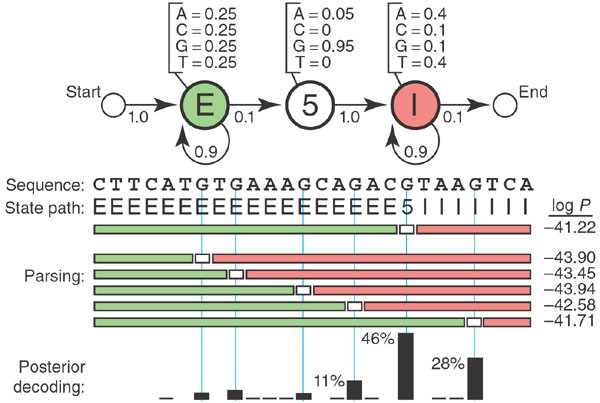
\includegraphics[draft=true, width=0.9\textwidth, trim={0 2.6cm 0 0}, clip=true]{Chapter_introduction/hmm}
    \else
        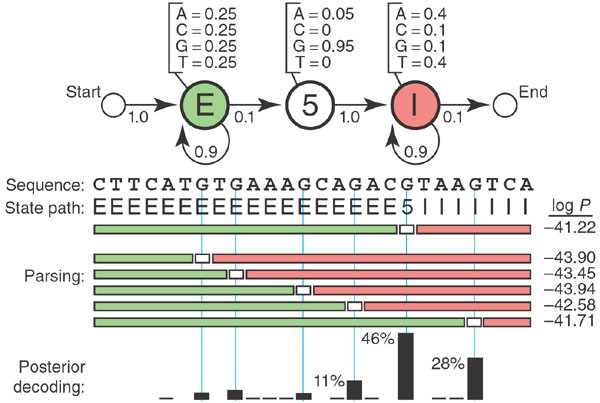
\includegraphics[width=0.9\textwidth, trim={0 2.6cm 0 0}, clip=true]{Chapter_introduction/hmm}
    \fi
    \caption{%
        Anatomy of a hidden Markov model (HMM) that models the sequence dependencies of a $5$' splice site in DNA.
        States for the exon (E), $5$' splice site and intron (I) are shown.
        Transition probabilities determine the paths that are allowed between the states, with one or more nucleotide in the exon, followed by the $5$' splice site at a G or A nucleotide, followed by one or more nucleotides in the intron.
        Emission probabilities are shown above the states that model the nucleotide composition of sequences in the three states.
        Nucleotides are emitted at every state visited on a path through the model from Start to End.
        Potential paths through the model for the `Sequence' are shown in the `Parsing' section, where the $5$' splice site state is a G or A.
        Log probabilities of paths are calculated by multiplying all transition and emission probabilities together and taking the logarithm.
        The most likely path is the path with the highest probability, in this case $\log P = -41.22$, which corresponds to the true `State path' for the sequence.
        Figure adapted from \cite{Eddy2004}.
    }
    \label{fig:hmm}
\end{figure}

HMMER \cite{Mistry2013} and HHsuite \cite{Steinegger2019} are the de facto standard tools to build HMMs and scan sequences against them. HHsuite can also perform pairwise HMM alignment \cite{Soding2005}, which can be thought of as comparing two MSAs. The jackhmmer program in HMMER, akin to PSI-BLAST, is an iterative search tool. Given a single query sequence and a target sequence database, an HMM is built from the sequence using a position-independent substitution matrix, such as BLOSUM62. Sequences in the target database are scanned against the HMM to identify hits, which are then aligned and used to build a new HMM. The whole process can be repeated for a few iterations to pull in ever more distantly related sequences.

\subsection{Structure homology}

We saw in the previous sections on sequence homology and HMMs that the sequence of amino acids---the primary protein structure---can be used to predict function. Therefore, sequence-function relationships exist. In this section, we extend this concept to structure-function and sequence-structure-function relationships \cite{Loewenstein2009,Lee2007,Watson2005}.

The primary protein structure can fold, which allows proteins to adopt higher order structures with many degrees of freedom. A $100$ residue protein, with $99$ peptide bonds, has approximately $3^{198} = 3\times 10^{95}$ stable $\phi$ and $\psi$ bond angle conformations \cite{Levinthal1969}. The polypeptide chain folds into local secondary structures \cite{Mizuguchi1995}, which arrange in space relative to each other in the tertiary structure. Multiple polypeptide chains can interact with each other in space to form the quaternary structure.

Higher order protein structures can be used to predict protein function \cite{Watson2005,Loewenstein2009}. The protein structure imparts knowledge about the 3D arrangement of amino acids to form functional sites in proteins, such as catalytic sites, regulatory motifs and allosteric sites \cite{Friedberg2006}.

Structure is more conserved than sequence \cite{Chothia1986}, which is perhaps to be expected, given the evolutionary need for proteins to be able to form stable arrangements in three-dimensional space.
Distantly related proteins, whose sequences have diverged considerably, so that they share lower sequence similarity than can be reliably detected using sequence comparison methods, may still be identified as homologues by comparison of their structures \cite{Lee2007}.
Therefore, structural homology can be used to predict protein function.
Conservation of structure between two proteins can be identified by measuring the root-mean-square deviation (RMSD) between equivalent atomic positions in two protein structures aligned in three-dimensional space.

CATH \cite{Sillitoe2019} (introduced in \ref{sec:intro-cath}) and SCOP \cite{Andreeva2020} classify domains into structurally-related homologous superfamilies, akin to Pfam for sequences. Both resources organise structures in a hierarchical taxonomy, that range from describing abstract structural features near the root, to specific structural features of superfamilies. Superfamilies are sub-classified into families in SCOP and functional families, or FunFams, in CATH (introduced in \ref{sec:intro-funfam}). Sequences in FunFams may not share high sequence identity, but critical residues---so called specificity-determining positions (SDPs)---will be conserved. This is not true for SCOP families, which are formed purely by sequence identity clustering. As such, SCOP families are more similar to `S60 clusters' (60$\%$ sequence identity clusters) of CATH superfamily domain sequences.

Knowledge of a protein's structure is neither necessary or sufficient to predict its function \cite{Grabowski2007,Loewenstein2009}. Historically, a protein's structure would be solved only after its function had been experimentally characterised. Like with sequence homology, care must be taken with transferring functions between structural homologues. Structural homology is sometimes sufficient for proteins to share function. However, some structures that have similar structures perform different functions. For example, the TIM barrel fold has a large pocket that has been exploited in multiple ways by introducing mutations in lining of the pocket that augment the function of the protein \cite{Glasner2006,Hannenhalli2000}. Over $27$ CATH superfamilies \cite{Sillitoe2019} contain a TIM barrel fold, covering $> 60$ different EC terms \cite{Lee2007}. Conversely, structural homology is not necessary for proteins to share function. Some proteins, like the many unrelated families of serine proteases, have separately evolved the catalytic triad via convergent evolution.

% % Remove stuff about function prediction
% Protein sequences, for which no structure is known, can be predicted using a wide-variety of structure prediction methods. Predicted structures can then be analysed using structure homology methods described here. One popular method for predicting structure is Phyre2 \cite{Kelley2015}. Other state-of-the-art methods for structure prediction will be discussed in \ref{sec:intro-applications}.

\subsection{CATH}
\label{sec:intro-cath}

CATH \cite{Orengo1999,Orengo1997,Sillitoe2019} classifies protein domain structures into evolutionarily related families, arranged in a four-level hierarchical taxonomy:

\begin{enumerate}
    \item \textbf{C}lass: secondary structure, all alpha-helical, all beta-sheet, mixed alpha-helical and beta-sheet, or little secondary structure.
    \item \textbf{A}rchitecture: global arrangement of secondary structure elements into the tertiary structure.
    \item \textbf{T}opology/fold: specific arrangement of secondary structure elements.
    \item \textbf{H}omologous superfamily: evidence of evolutionary relatedness of domains.
\end{enumerate}

The current version of CATH (v4.2) contains \num{6119} superfamilies. To identify these groups, protein structures are aligned using SSAP (structure and sequence alignment program) \cite{Taylor1989}. SSAP employs double-dynamic programming to extend the concept behind Needleman and Wunsch's sequence alignment algorithm \cite{Needleman1970} to 3D protein structures. As such, the double-dynamic programming method is guaranteed to find the optimal alignment of any two given proteins. The algorithm was subsequently modified to align structural motifs \cite{Orengo1993}, akin to Smith and Waterman's adaptation of the global sequence alignment algorithm to find local matches \cite{Smith1981}.

Crucial to its success is the way that SSAP represents protein structures. Instead of using the letters of the amino acid alphabet, SSAP uses interatomic vectors between the C$\beta$ atoms of all residues, except glycines. The inclusion of positional information proved key to SSAP's success over contemporary methods that only considered interatomic distances \cite{Orengo1996}. Furthermore, interatomic vectors proved to be necessary and sufficient to align protein structures \cite{Taylor1989a}. Inclusion of additional structural information improved alignments in only the most challenging cases \cite{Taylor1989a}.

In 1993, there were structures of \num{1800} chains in the PDB. Because $\sim 50$ new structures were being deposited each month, it became obvious that an automated method would be needed to identify protein folds and classify proteins into protein fold families. SSAP was initially used to align proteins containing globin domains that have very low sequence similarity, but were found to conserve the same domain structure \cite{Taylor1989}. SSAP was subsequently used to identify families of protein folds in groups of proteins with similar sequences \cite{Orengo1993a}. These families established the foundations of CATH \cite{Orengo1999,Orengo1997}.

CATH can be used for protein function prediction in a number of ways. Firstly, CATHEDRAL \cite{Redfern2007} can be used to align a query structure to structure representatives from each superfamily. Functions of proteins within any matching superfamilies can be transferred. However, this classification is usually too broad to provide fine-grained functions. Secondly, CATH-Gene$3$D can be used to assign a protein sequence to CATH superfamilies (see \ref{sec:intro-gene3d}). Finally, CATH-FunFams can be used to assign a protein sequence to FunFams (see \ref{sec:intro-funfam}). Next, we introduce these two methods Gene$3$D and FunFams.

\subsubsection{Gene$3$D}
\label{sec:intro-gene3d}

Gene$3$D \cite{Lees2012,Lees2014,Lewis2018} allows CATH superfamily domains to be predicted in protein sequences, using sequence information alone. Gene$3$D exploits protein sequence-structure relationships by representing the sequence diversity of each CATH superfamily as a set of one or more HMMs. Sequences are scanned against these HMMs and assigned to any matching superfamilies. Interestingly, Gene$3$D is a hybrid sequence-structure-homology method because structures are used to define the domain boundaries of domain sequences.
The equivalent functionality of Gene$3$D is provided to SCOP via the SUPERFAMILY database \cite{Pandurangan2019}.

To construct Gene$3$D's HMMs, domain sequences within a CATH superfamily are first clustered at S$95$ using CD-HIT \cite{Fu2012}, aligned and an HMM is built using jackhmmer's iterative search functionality \cite{Mistry2013}. UniProt is searched using this HMM and any sequences that meet the HMM inclusion threshold are retained. A second iteration of jackhmmer is then performed. The HMM from the second iteration is used if the ratio of true positive predictions improves, otherwise the HMM from the first iteration is used.

Gene$3$D supports the identification of discontinuous domains. Discontinuous domains can form as the result of insertion events, whereby a continuous domain becomes discontinuous when a domain is inserted between its start and stop positions. To improve their identification, HMMs are built for discontinuous domains by also including the inserted domain sequences.

In any given protein sequence, there may be many, overlapping, matches to S$95$ models from the same, or different CATH superfamilies. cath-resolve-hits \cite{Lewis2019} is used to reduce the set of matches to an optimal subset of non-overlapping matches (\ref{fig:crh}). The algorithm uses dynamic programming to deterministically find the set of domains that maximises the sum of the bit scores.

\begin{figure}[!hbt]
    \centering
    \ifredact
        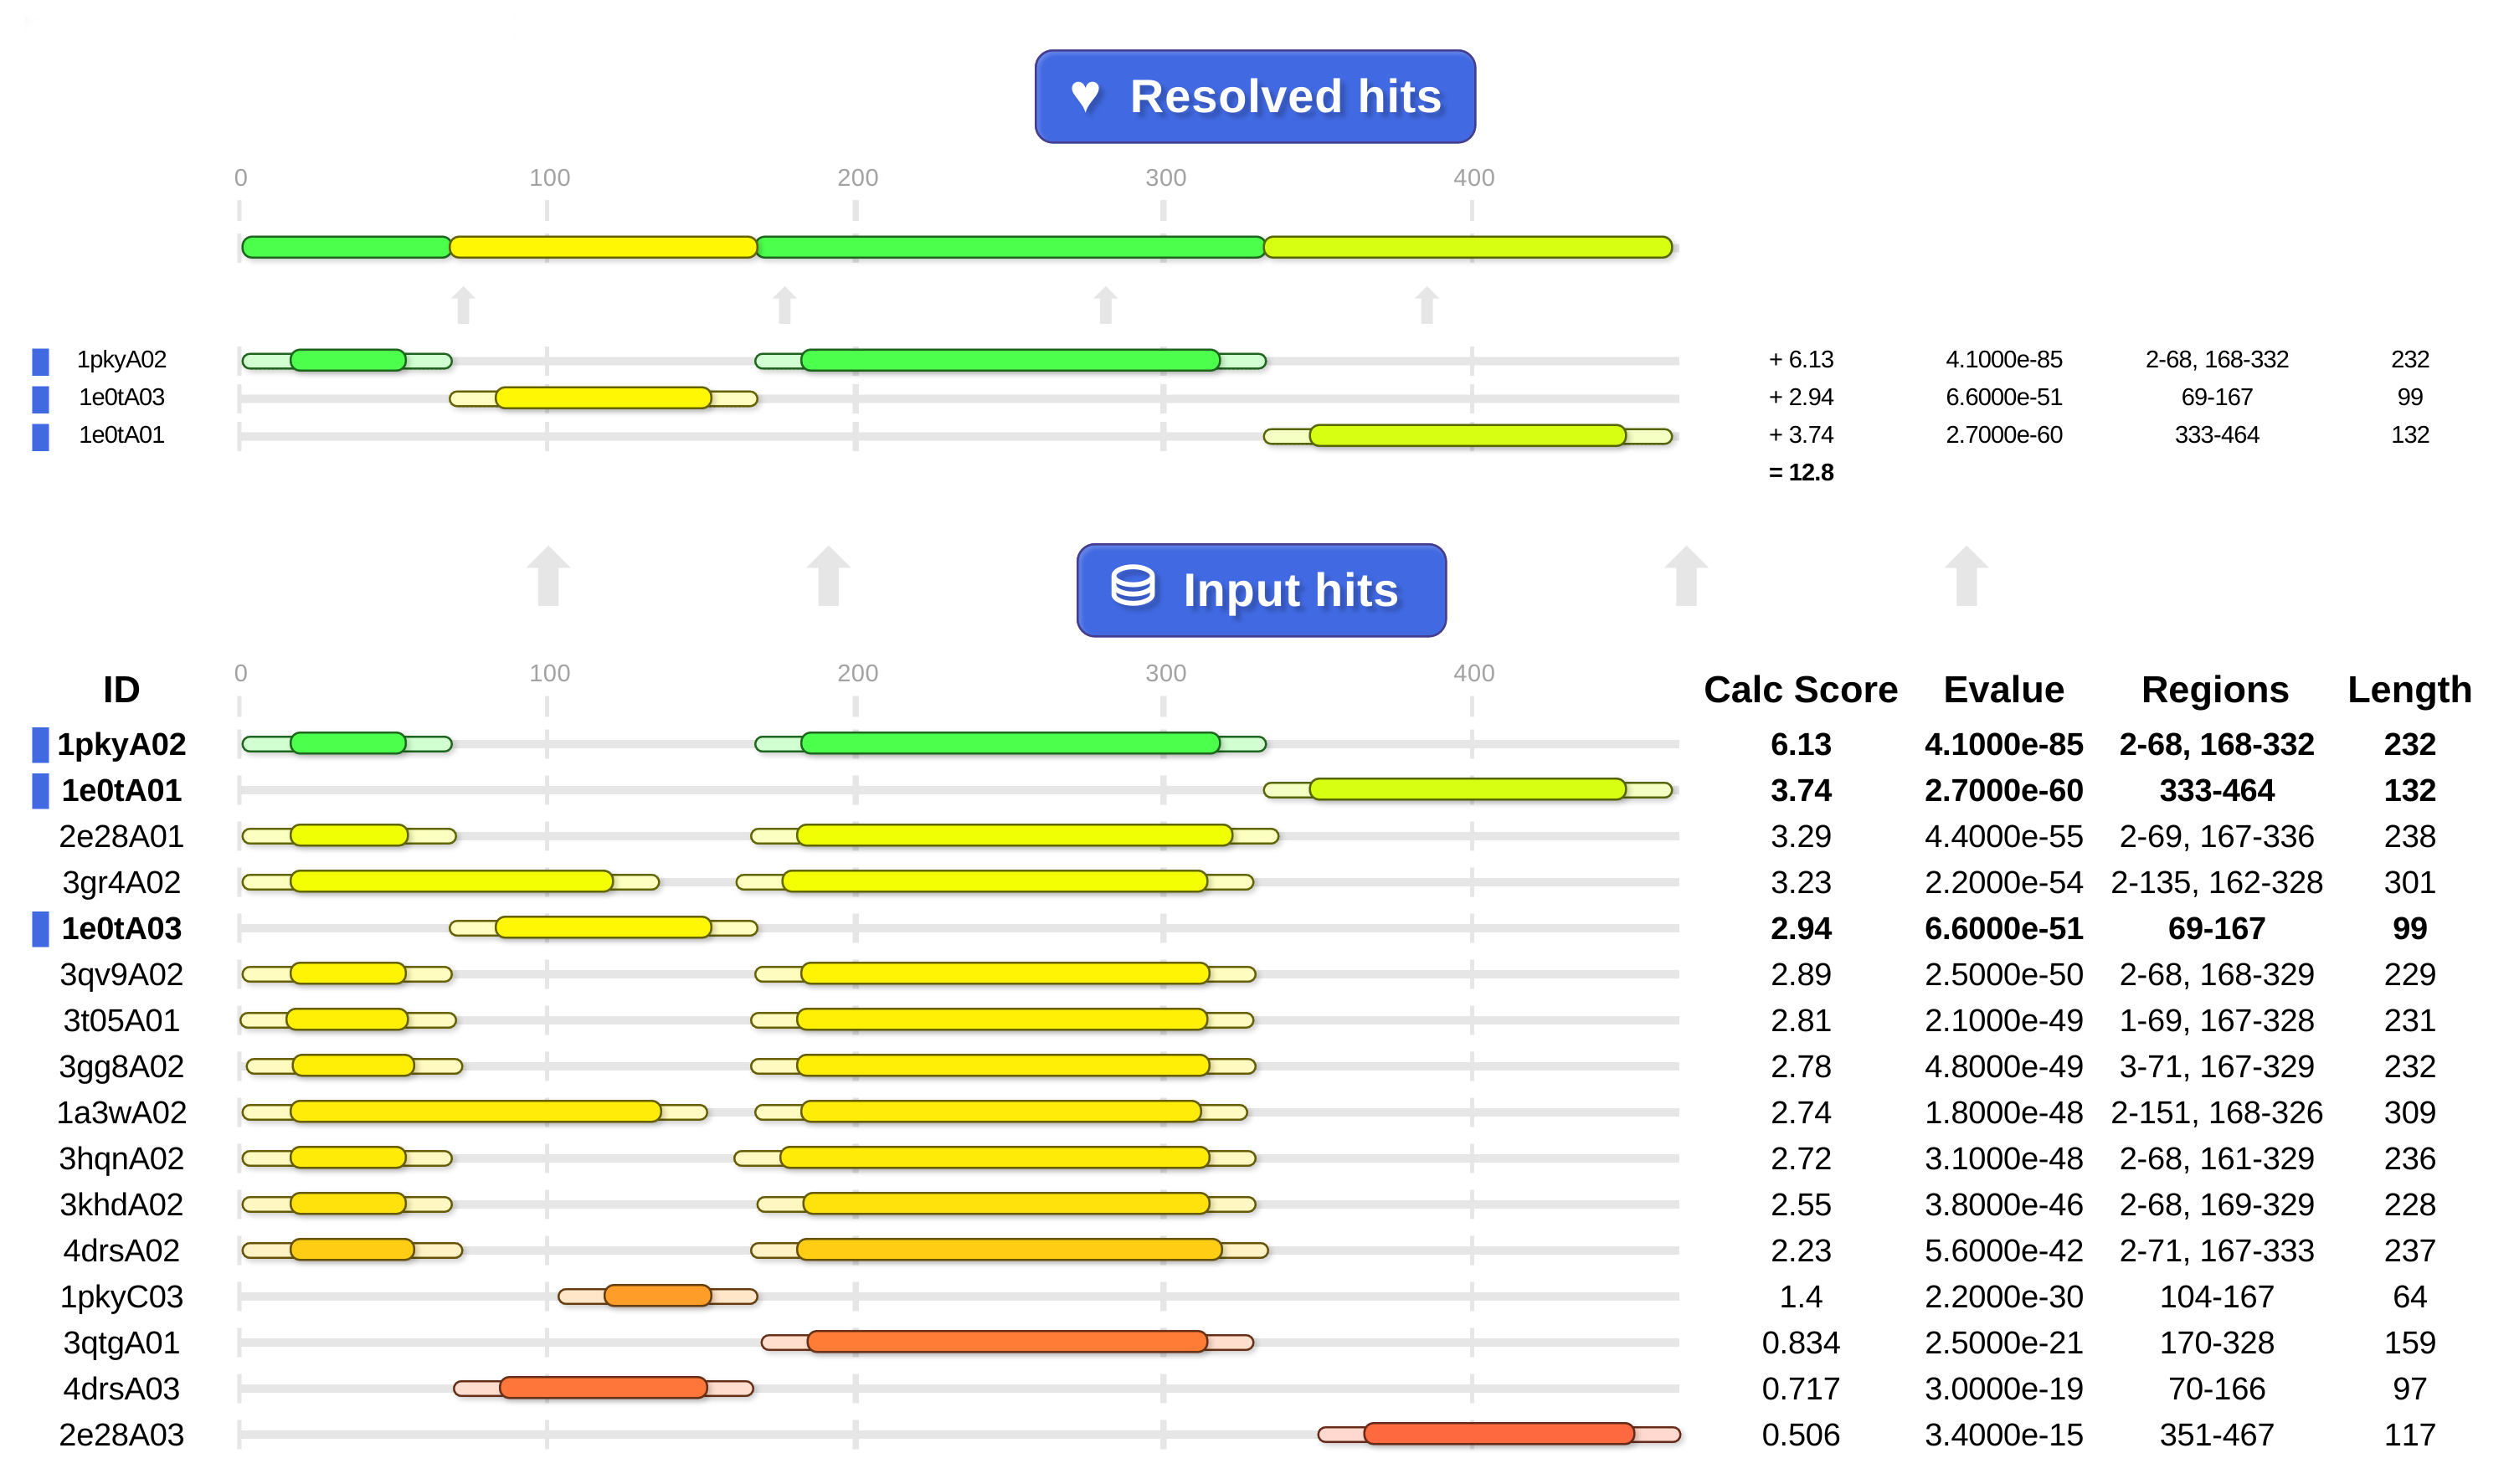
\includegraphics[draft=true, width=0.9\textwidth]{Chapter_introduction/crh}
    \else
        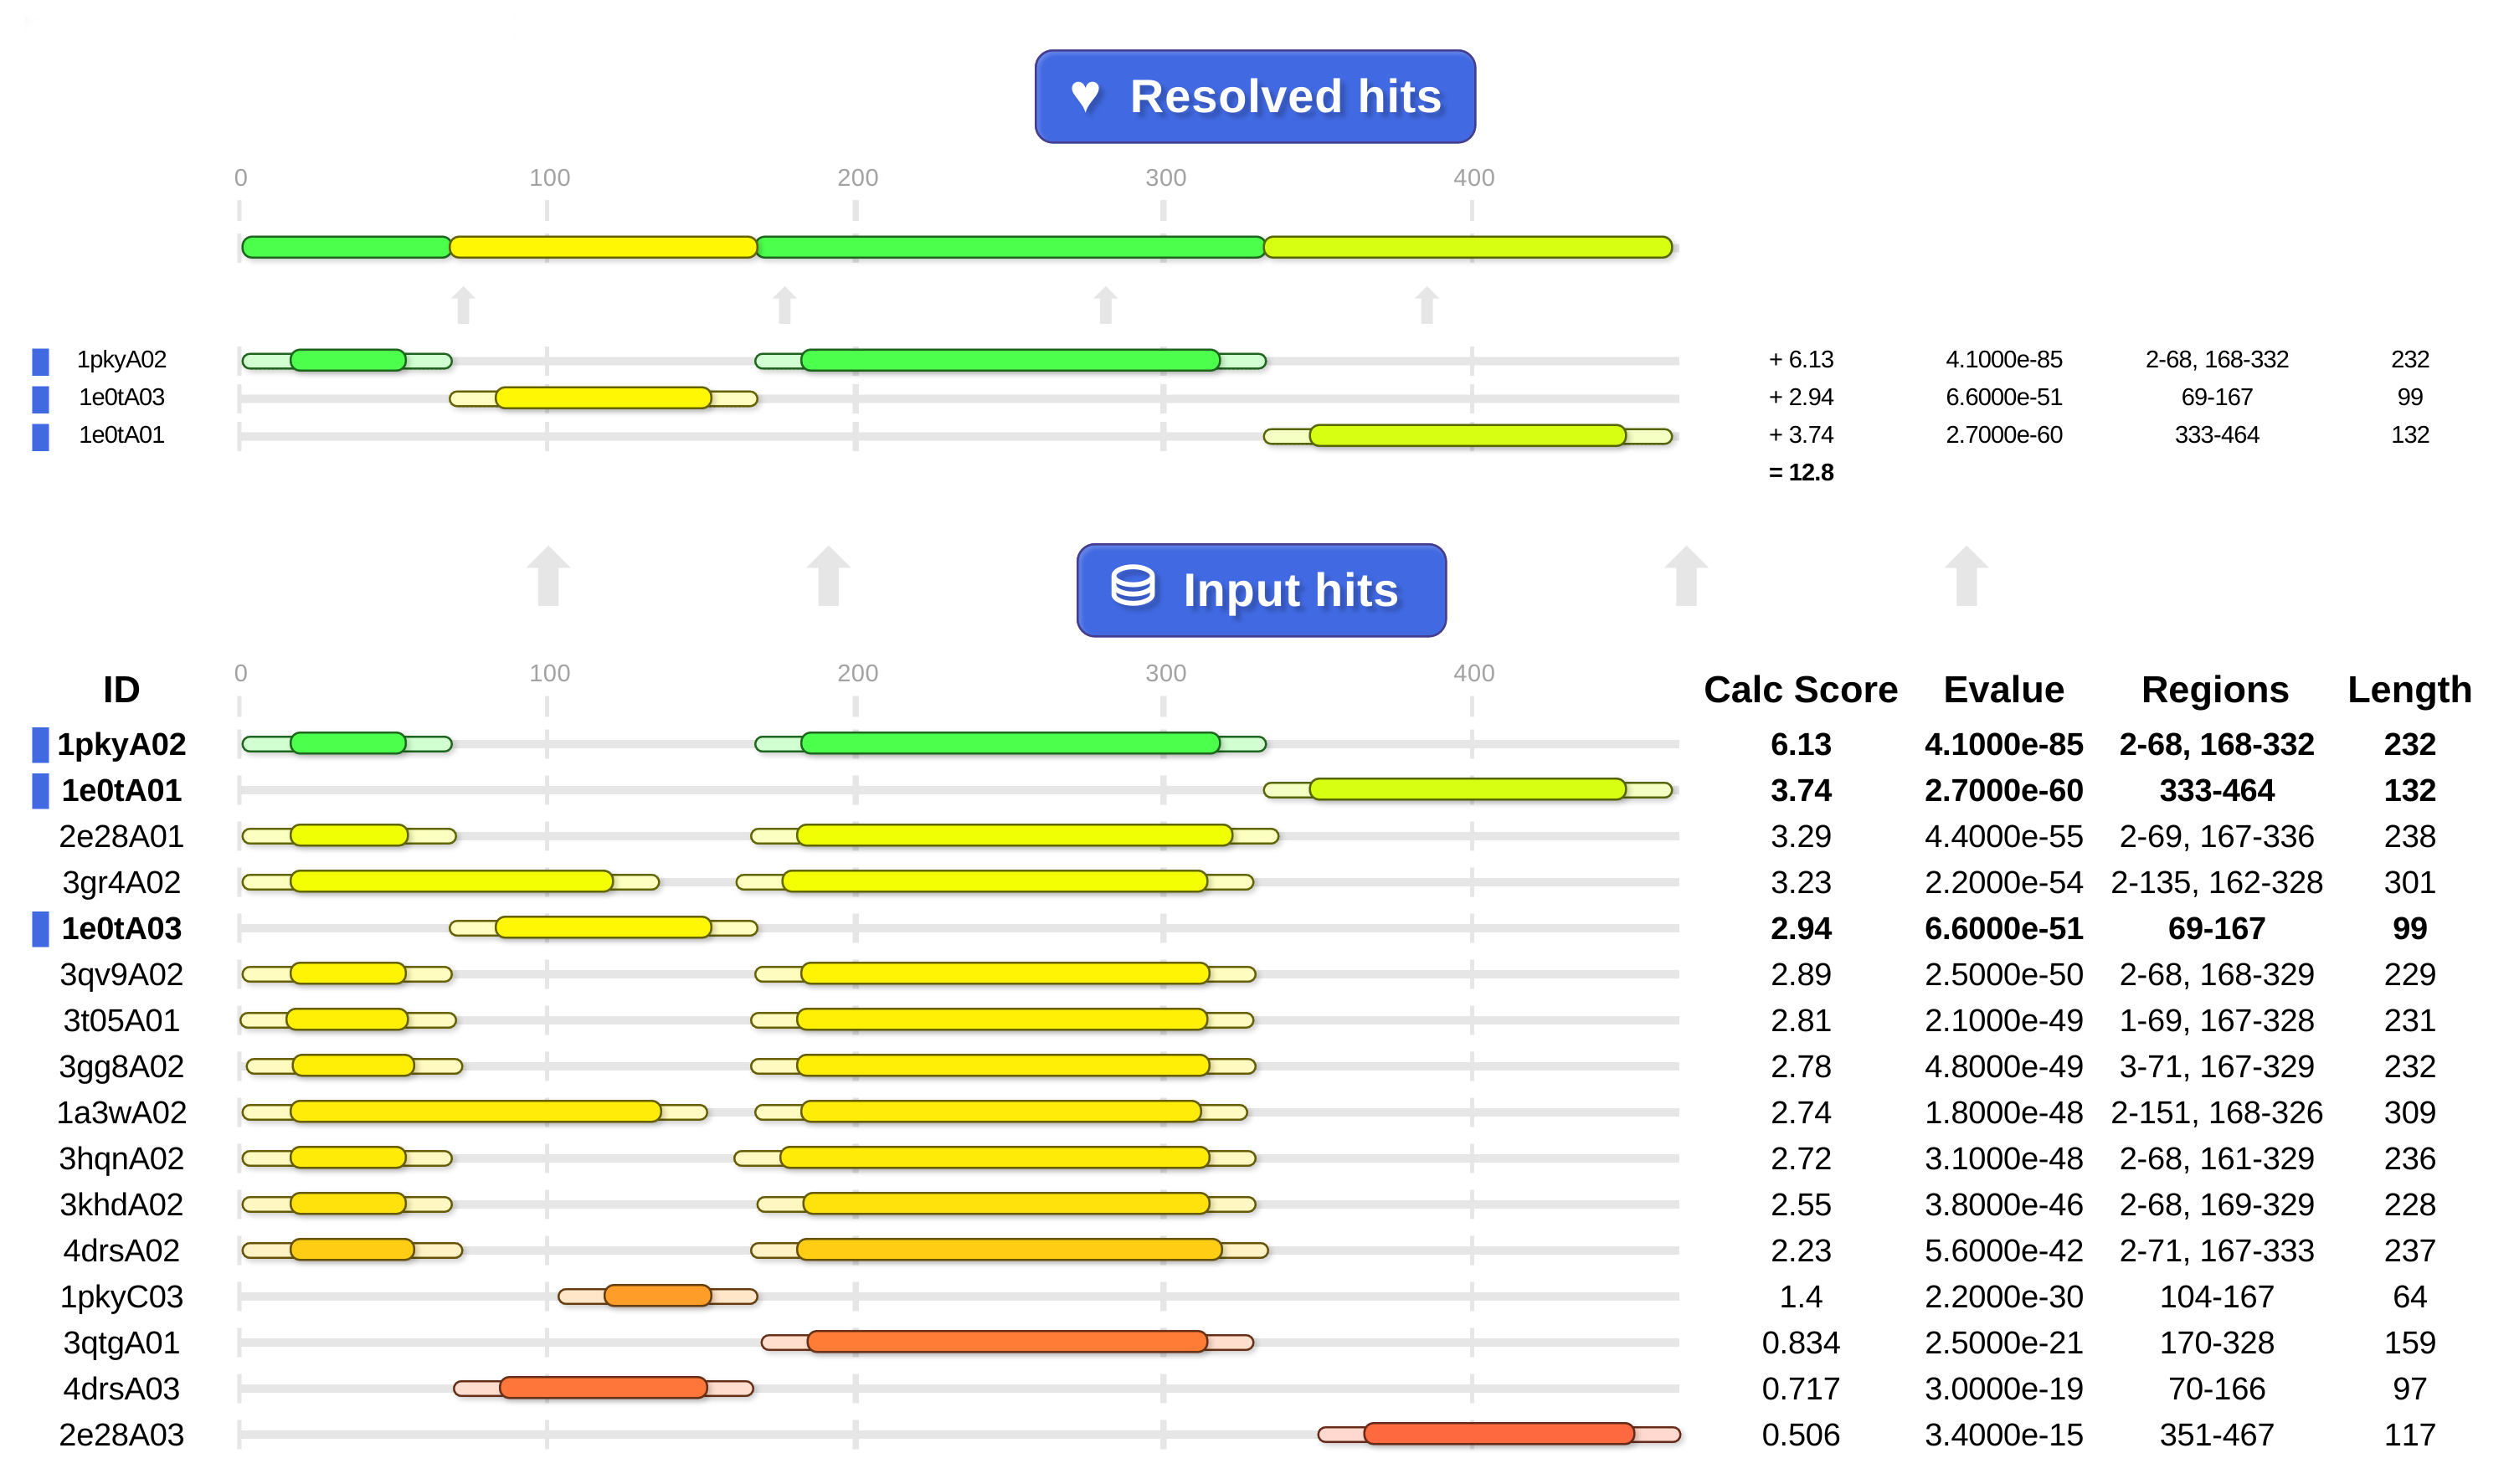
\includegraphics[width=0.9\textwidth]{Chapter_introduction/crh}
    \fi
    \caption{%
        cath-resolve-hits resolves the domain boundaries of multiple `Input Hits' to an optimal subset of non-overlapping `Resolved Hits' that form the MDA.
        Figure taken from https://cath-tools.readthedocs.io/en/latest/tools/cath-resolve-hits/.
    }
    \label{fig:crh}
\end{figure}

\subsubsection{FunFams}
\label{sec:intro-funfam}

FunFams are groups of homologous proteins that perform the same function, or functions. SDPs are used to identify and group likely isofunctional proteins into FunFams. Sequences in CATH superfamilies are sub-classified into fine-grained groups, according to sequence alone. The current version of CATH (v4.2) contains \num{67598} FunFams in \num{2620} of the \num{6119} superfamilies. Whilst FunFams are strictly a type of sequence-homology method, the sequences used to construct CATH-FunFams are from Gene$3$D hits, so are structural homologues. FunFams were only made possible because Gene$3$D is now able to retreive millions of sequence homologues from UniProt. Having said this, FunFam is a general sequence-based protocol that can be applied to any protein family. In addition to CATH-FunFams, we also generate Pfam-FunFams from Pfam families. 

FunFams are generated in a four step process:

\begin{enumerate}
    \item
        \textbf{Sequences containing Gene$3$D predictions of a particular superfamily domain are separated by MDA and clustered at S$90$}

        Clusters that do not have any experimental GO terms associated are removed. The remaining clusters are referred to as starting clusters. Clusters that are not associated with any experimentally characterised functions are removed for practical---not scientific---reasons. Removing these functionless clusters helps to reduce the total number of starting clusters, to fit within memory limits. Given unlimited memory, or a low-memory method of generating FunFams, FunFams could be generated using all S$90$ clusters. This would mean that some FunFams would not have any associated functions, but these could always be added \emph{post hoc} once any one of the FunFam's members became experimentally characterised.

    \item
        \textbf{GeMMA \cite{Lee2009} is a greedy algorithm that builds a neighbour-joining tree by bottom-up hierarchical agglomeration}

        Given $n$ starting clusters, GeMMA makes $n-1$ merges. Leaves and internal nodes in the tree are clusters of related superfamily domain sequences, represented as HMMs (\ref{fig:gemma_funfhmmer}). To decide which node to merge at each of the $n-1$ steps, HMMs are aligned pairwise and the closest pair of clusters are merged. The merged set of sequences are aligned, a new HMM is generated and the merging process is repeated.

        \begin{figure}[!hbt]
            \centering
            \ifredact
                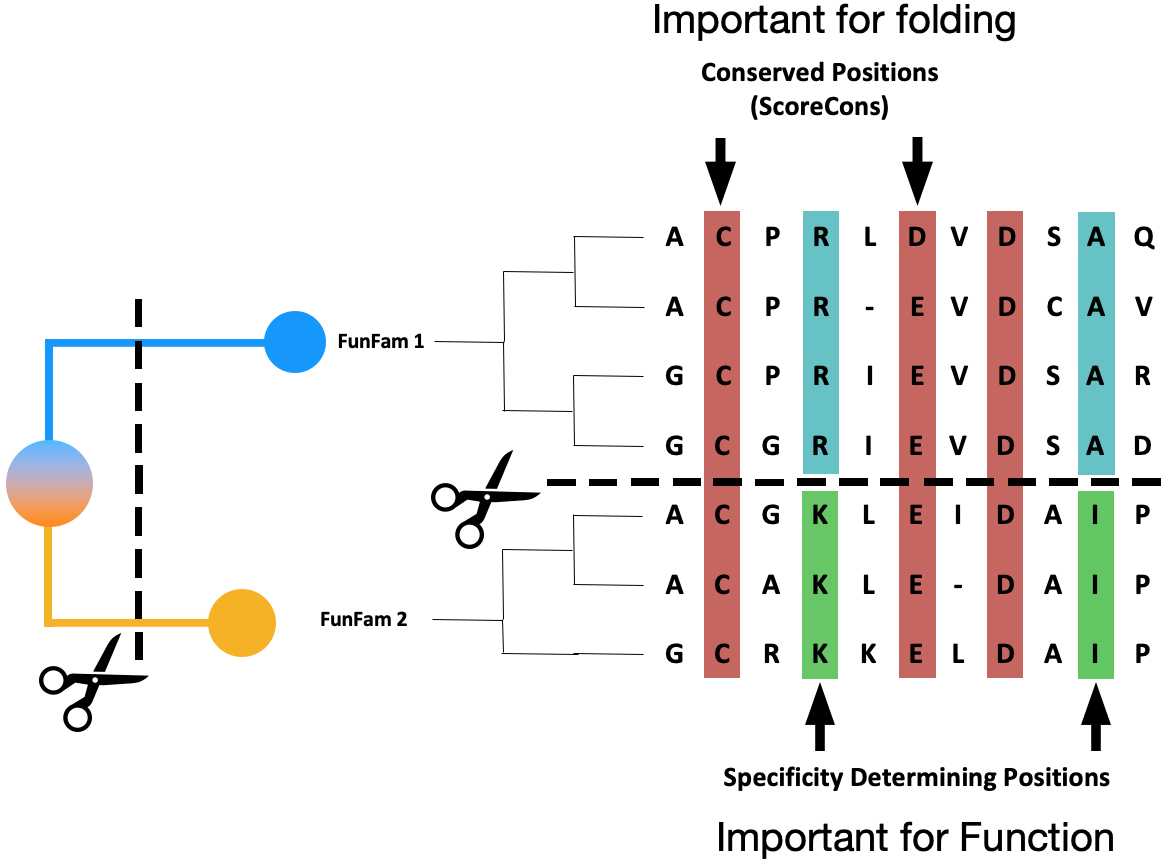
\includegraphics[draft=true, width=0.8\textwidth, trim={0 2cm 0 2cm}, clip]{Chapter_introduction/gemma_funfhmmer}
            \else
                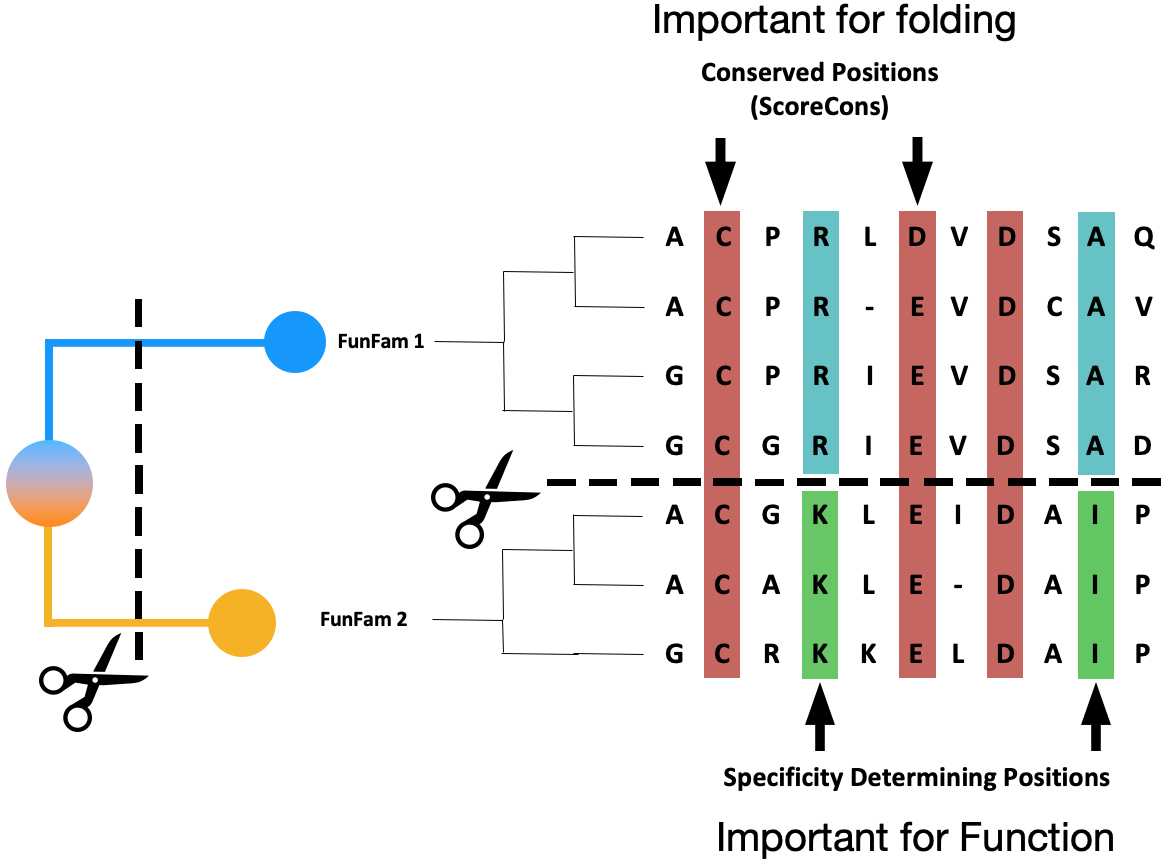
\includegraphics[width=0.8\textwidth, trim={0 2cm 0 2cm}, clip]{Chapter_introduction/gemma_funfhmmer}
            \fi
            \caption{%
                An overview of the GeMMA and FunFHMMer algorithms.
                Scissors denote the points where the FunFHMMer algorithm cuts the GeMMA tree.
                Specificity-determining positions are identified using GroupSim (\ref{fig:groupsim}).
                Figure courtesy of Nicola Bordin.
            }
            \label{fig:gemma_funfhmmer}
        \end{figure}

        Generally, we have noticed that the upper bound of starting clusters is \num{5000} before reaching the memory limits of our largest machines (with $3$ TB memory). GeMMA used to be applied to an entire superfamily \cite{Lee2009}. As superfamilies have grown in size, the protocol was changed so that GeMMA is run on subsets of proteins that have the same MDA (see \ref{sec:intro-gardener}). Partitioning superfamilies by MDA makes biological sense because the MDA is a determinant of function \cite{Yu2019,Lees2014,Bashton2007}. Proteins with different MDAs are unlikely to be in the same FunFam, so it is reasonable to segregate them \emph{ab initio}.

    \item
        \textbf{FunFHMMer \cite{Das2015b} determines the optimal partitioning of the GeMMA tree into clades, each of which is a FunFam}

        FunFHMMer operates on MSAs of leaves and internal nodes (\ref{fig:gemma_funfhmmer}). Diverse protein sequences are required for FunFHMMer to elucidate conservation patterns and SDPs in MSAs. FunFHMMer traverses the GeMMA tree from the leaves towards the root. Let $v_i$ and $v_j$ be two child nodes that are connected to a parent node $v_p$. A functional coherence index is calculated for $v_p$ to determine whether the tree should be cut before $v_p$ (traversing in the direction from leaf to root). If the tree is cut before $v_p$, two FunFams $F_1$ and $F_2$ are produced, where $F_1 = v_i$ and $F_2 = v_j$. Otherwise, if the tree is subsequently cut after $v_p$, $v_i$ and $v_j$ will form part of the same FunFam $F$, $\{v_i \cup v_j\} \subseteq F$. The functional coherence index is powerful, generates functionally pure FunFams and imbues FunFams with their predictive power. The index considers three parameters:

        \begin{itemize}
            \item
                Information content of the MSA. Calculated using the diversity of position scores (DOPS) from ScoreCons \cite{Valdar2002}. MSAs with DOPS $> 70$ are generally considered to be sufficiently diverse.
            \item
                Proportion of predicted SDPs in an MSA. SDPs are predicted using GroupSim (\ref{fig:groupsim}), which calculates a score for each position in an MSA, whose sequences are pre-assigned into two groups according to the sequences in the child nodes \cite{Capra2008}. The SDP-to-conserved position ratio determines whether the tree is cut.
            \item
                Gaps in an MSA. Gaps in the parent alignment indicate that the child alignments were of different lengths. A multiplicative factor of $0$ results if the number of gap positions is greater than the number of non-gap positions.
        \end{itemize}

        Some residues that are necessary for the function of a protein, such as catalytic residues in the active site of an enzyme, may be highly conserved in a set of S$90$ clusters. Whilst these residues may be predictive of the general function of a given protein, they do not determine how the GeMMA tree is partitioned by FunFHMMer into FunFams. Only differentially conserved residues determine the partitioning of the tree, and therefore the functional specificity of FunFams. Highly-conserved residues may also be useful for protein structure prediction, particularly for evolutionary covariation techniques \cite{Marks2011,Senior2020}.

        \begin{figure}[!hbt]
            \centering
            \ifredact
                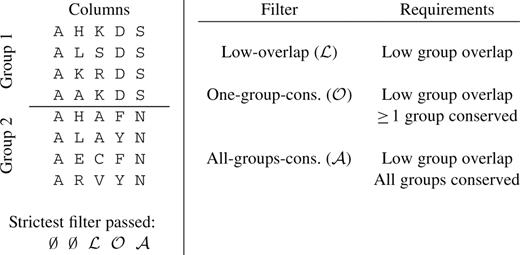
\includegraphics[draft=true]{Chapter_introduction/groupsim}
            \else
                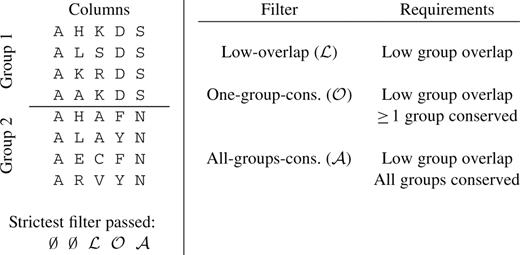
\includegraphics{Chapter_introduction/groupsim}
            \fi
            \caption{%
                GroupSim predicts specificity-determining positions (SDPs) in alignments.
                Each column in the alignment is assigned to one of four sets, explained on the right of the figure,
                where $\emptyset$ denotes the empty set.
                Figure taken from \cite{Capra2008}.
            }
            \label{fig:groupsim}
        \end{figure}

    \item
        \textbf{Generate full FunFams}

        The FunFams generated by the previous step are known as the seed alignments.
        Seed alignment sequences are then scanned against their corresponding HMM to assign an inclusion threshold to each FunFam, which is the largest E-value for the worst match.
        Full alignments for FunFams are generated using sequences from the superfamily that were in S$90$ clusters without an experimental GO term. These sequences are scanned against the seed HMMs using the per FunFam inclusion thresholds. Sequences are assigned to any matching FunFam, but if sequences match to multiple FunFams, they are assigned to the best matching FunFam.
\end{enumerate}


\subsubsection{GARDENER}
\label{sec:intro-gardener}

The FunFam generation protocol has recently been improved in a new algorithm, GARDENER, which performs two rounds of FunFamming, rather than the single round in the original protocol set out above (\ref{fig:gardener}). In the first round, GARDENER processes each MDA partition separately using GeMMA and FunFHMMer to generate FunFams. These initial FunFams, from all of the MDA partitions, are then pooled. Initial FunFams are then treated as starting clusters for a second round of GeMMA and FunFHMMer. The FunFams from the second round of FunFamming are used as FunFams for the superfamily. Note that if a superfamily has a single MDA, then only one round of GeMMA and FunFHMMer are performed, instead of two. GARDENER is advantageous because it allows over-split FunFams and singleton FunFams, from the first round, to be merged in the second round. GARDENER is explained in more detail in \ref{methods:fran}.

\begin{figure}[!hbt]
    \centering
    \ifredact
        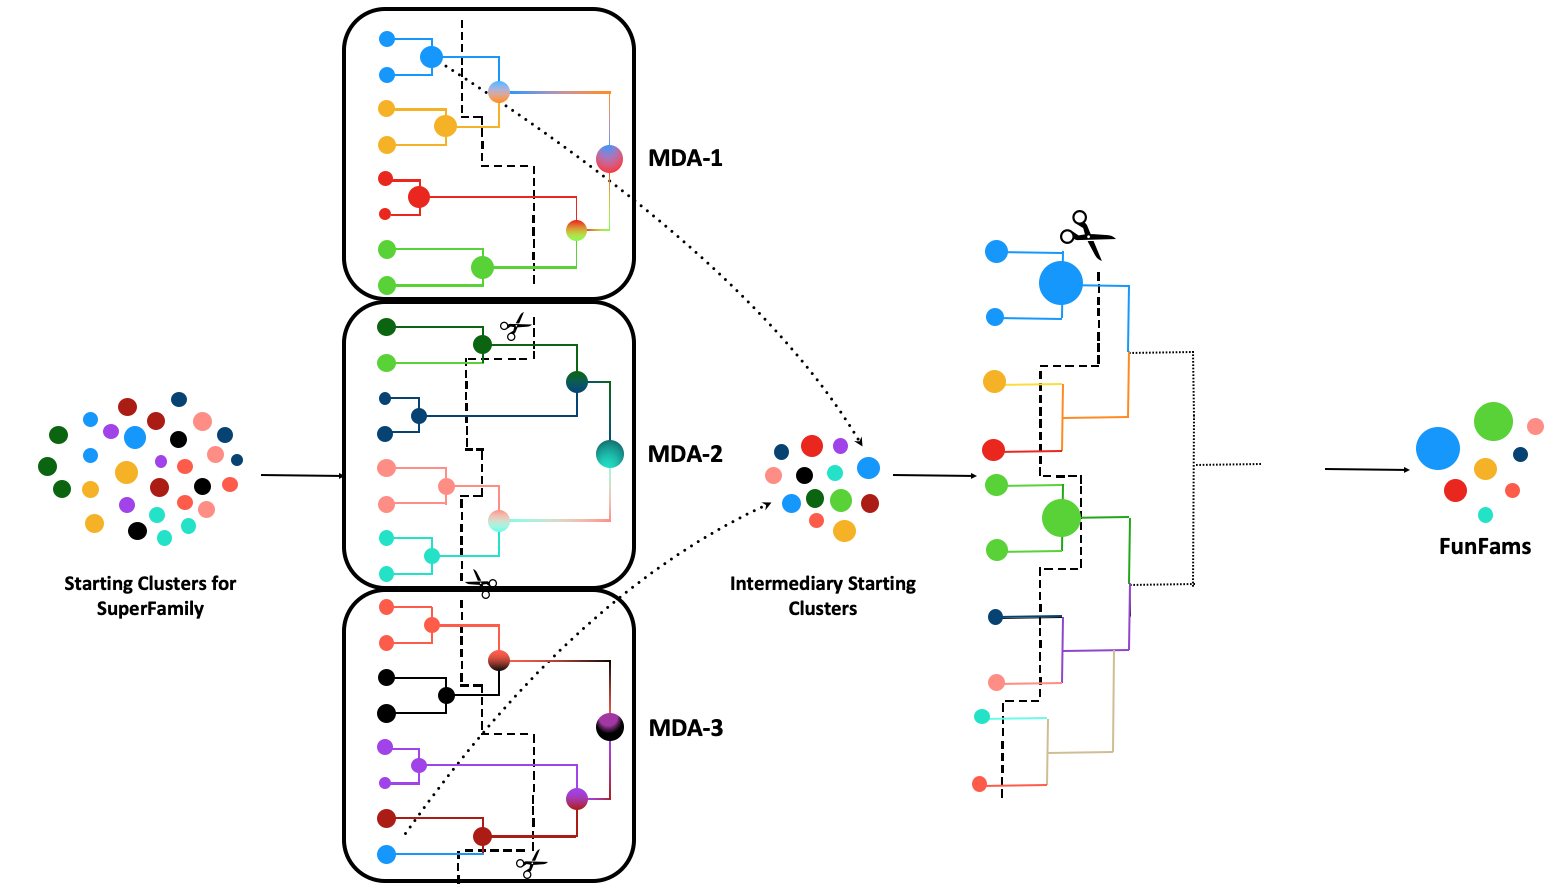
\includegraphics[draft=true, width=\textwidth]{Chapter_introduction/gardener}
    \else
        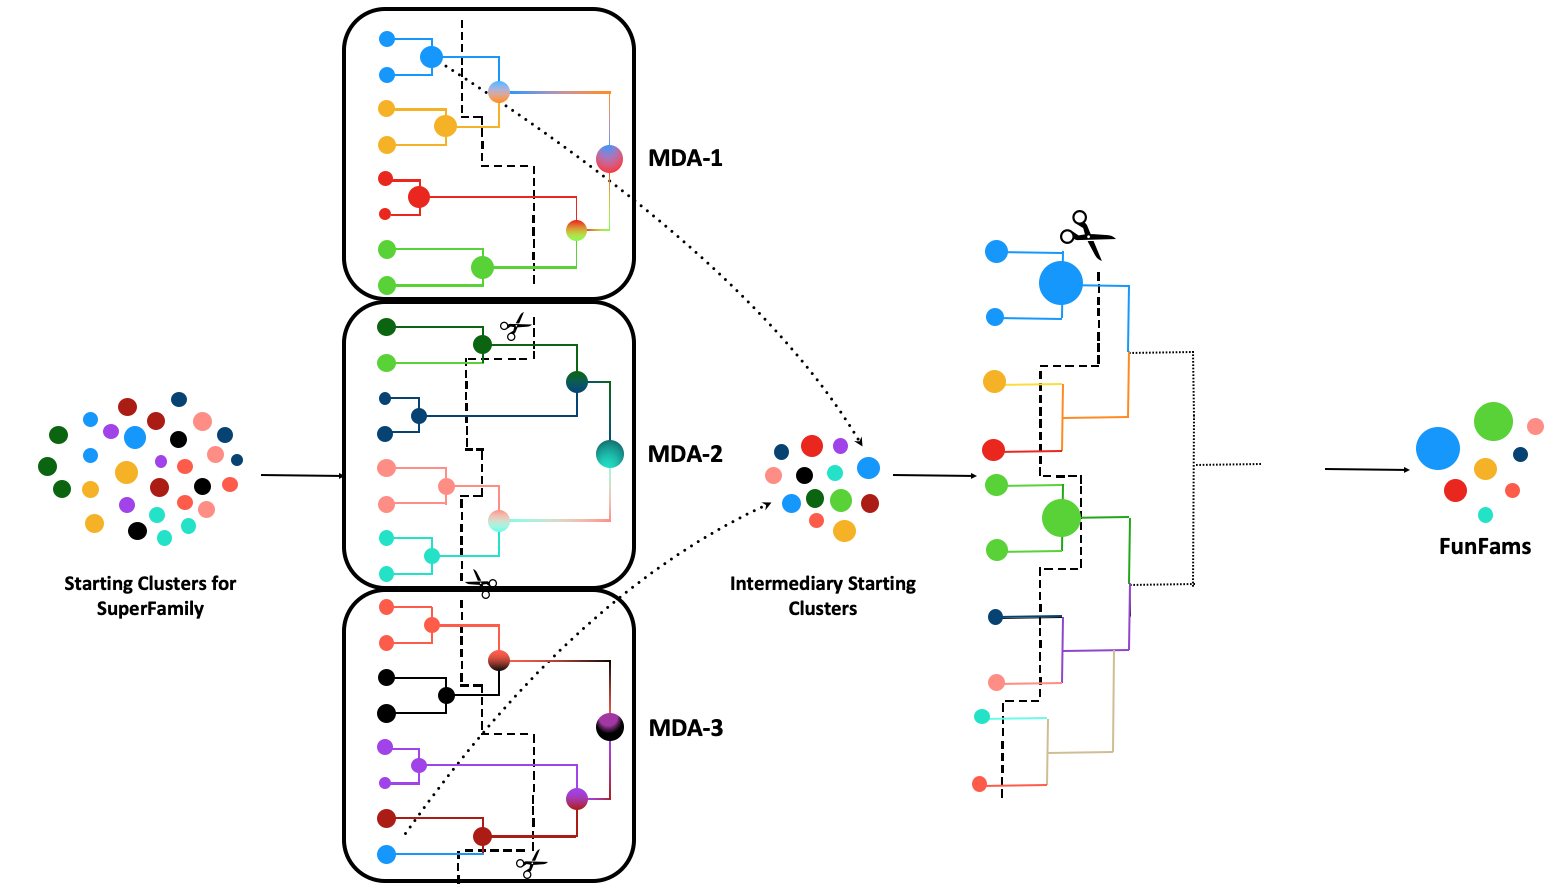
\includegraphics[width=\textwidth]{Chapter_introduction/gardener}
    \fi
    \caption{%
        An overview of the GARDENER algorithm.
        Scissors denote the points where the FunFHMMer algorithm cuts the GeMMA tree.
        Figure courtesy of Nicola Bordin.
    }
    \label{fig:gardener}
\end{figure}

\subsection{Symbolic representations of functions}

So far, we have been referring to functions as abstract concepts (\ref{sec:intro-function}). Here, we introduce data structures that are used to represent functions symbolically. In recent years, natural language processing of unstructured text has become increasingly powerful, but for computational and curational ease, functions are best represented in a structured way. These data structures must represent the set of all possible functions (or all known functions), rather than assigning functions \emph{ad hoc} \cite{Lee2007}. One way to do this is using a `controlled vocabulary' for the set of all possible functions.

We have already noted that functions are related to each other (\ref{sec:intro-pre-bioinformatics-age}). Some functions are more closely related to some than to others. As such, controlled vocabularies of functions lend themselves naturally to being organised in hierarchical, tree-like structures. The Enzyme Commission (EC) \cite{Bairoch2000} uses a simple four-level hierarchy, where child terms are strict descendants of one parent term. Child terms describe more specific functions that are a subset of the parent function. For example, the function of tripeptide aminopeptidases are described by the EC number ``EC 3.4.11.4'', where the four levels correspond to:

\begin{itemize}
    \item EC 3 hydrolases
    \item EC 3.4 peptidases
    \item EC 3.4.11 N-terminal exopeptidases
    \item EC 3.4.11.4 N-terminal exopeptidase for tripeptides
\end{itemize}

\num{7936} different enzymatic functions have been described using the EC database.
These terms have been annotated \num{246858} times to a total of \num{235086} protein IDs from direct experimental characterisation of an enzyme's activity, reactants, products, cofactors and specificities.

Whilst EC terms are focussed on enzyme function, the Gene Ontology (GO) GO \cite{Carbon2018} is a more ambitious project than EC, in that it aims to characterise molecular function, biological processes and subcellular location of proteins.
So far, the GO describes \num{44167} functions, across three disjoint namespaces: `biological process' (BP), `molecular function' (MF) and `cellular component' (CC).
Proteins from \num{4728} species have been characterised using a total of \num{8047744} GO annotations to \num{1569827} unique proteins.
We use the GO extensively in this thesis and attempt to increase the functional coverage of proteins by predicting GO term annotations.

% total terms

% grep -c "^ID" enzyme.dat

% total IDs

% grep "^DR" enzyme.dat | grep -o ";" | wc -l

% unique IDs

% open(joinpath(@__DIR__, "enzyme.dat")) do f
%     ids = Set{String}()
%     for line in eachline(f)
%         if startswith(line, "DR")
%             line = replace(line, "DR"=>"")
%             # line = replace(line, ";"=>"")
%             l = split(line, ";")
%             for id in l
%                 push!(ids, id)
%             end
%         end
%     end
%     return ids
% end

`Ontology' is the branch of philosophy that deals with the nature of being, of which there are many possible relationships.
Describing these relationships requires a more flexible data structure than the tree used in EC.
The GO uses a directed acyclic graph (DAG) (\ref{fig:go}), where edges in the graph are directed from child terms to parent terms.
The DAG is actually a multi-DAG (a DAG with multiple edge types), used to represent one-to-many relationships between functions.
Possible relationships in the GO DAG include `is a', `part of' and `regulates'.
For example, `6-phosphofructokinase activity' is part of `glycolytic process through fructose-6-phosphate', which can be positively and negatively regulated.
Multiple levels of functions can be queried using the GO, for example, it can be used to find all genes in a genome that are involved in signal transduction, or one can focus only on the subset of genes that are tyrosine kinases.

\begin{figure}[!hbt]
    \centering
    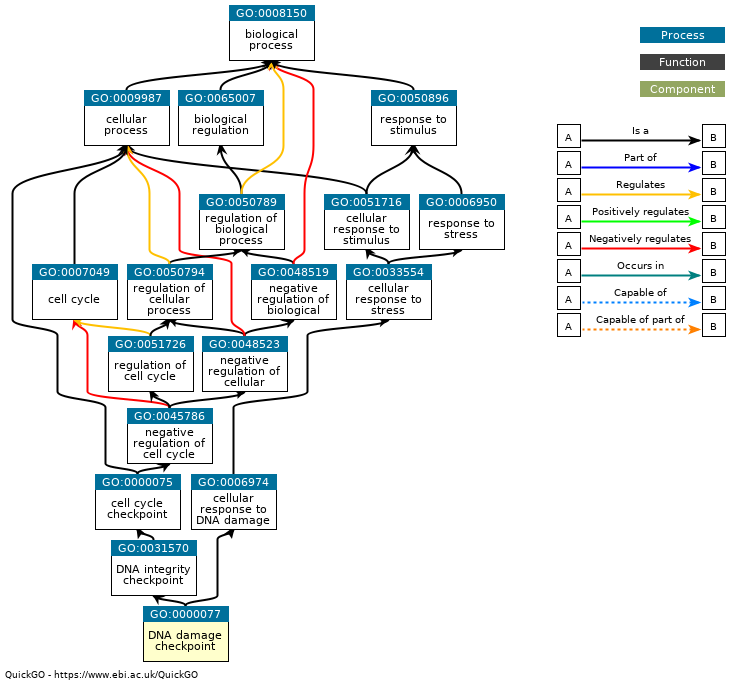
\includegraphics[width=0.8\textwidth]{Chapter_introduction/go}
    \caption{%
        The Gene Ontology.
        Subgraph of the Gene Ontology for `DNA damage checkpoint' (GO:0000077).
        Figure taken from https://www.ebi.ac.uk/QuickGO/term/GO:0000077.
    }
    \label{fig:go}
\end{figure}

Whereas EC annotations are based on direct experimental characterisation, and therefore should be trustworthy, GO introduces a notion of quality via its evidence codes attached to each annotation of a GO term to a protein.
Evidence codes can be broadly categorised into groups, with functions assigned by:
direct experiment (EXP, IDA, IPI, IMP, IGI and IEP) and their high-throughput counterparts (HTP, HDA, HMP, HGI and HEP); 
inferred phylogenetically (IBA, IBD, IKR and IRD) or computationally (ISS, ISO, ISA, ISM, IGC and RCA);
assigned by a curator (IC);
automatically inferred annotations (IEA);
and low-quality, untrusted annotations without evidence to back them up (NAS, ND).
These groups are approximately ordered by how much confidence one would assign to an annotation with that evidence code.

A number of other protein function databases are touched on in this thesis, including the MIPS FunCat database \cite{Pagel2005,Ruepp2004}; the Human Phenotype Ontology \cite{Kohler2019}, used to annotate proteins that cause phenotypic abnormalities in human diseases; and the Disorder Ontology \cite{Hatos2020} that characterises intrinsically disordered proteins.
FunCat was developed during the initial sequencing of the \emph{Saccharomyces cerevisiae} genome to describe yeast protein function.
Similar to the EC, MIPS terms are a controlled vocabulary arranged in a three-layer hierarchy of increasing functional specificity.
Despite MIPS being rather an ancient resource, we use some of its annotations in \ref{chapter:network-fusion} to benchmark our method against two other methods that chose to use MIPS \cite{Cho2016,Gligorijevic2018}.
Although we do not use the Human Phenotype Ontology and the Disorder Ontology, we encounter them in \ref{chapter:yeast} as part of the CAFA 4 evaluation of protein function prediction methods.

Now that we know how functions are represented computationally, next we introduce how to compare the predictive performance of different methods on the same prediction task.

\subsection{Benchmarking performance}

Many methods have been developed to predict protein function, each often claiming to be the state-of-the-art. Such claims should always be treated with suspicion due to disingenuous science, overfitting on evaluation data, or luck. Transparent, public benchmarks are required to evaluate different methods within a community. Protein structure prediction first introduced the CASP \cite{Kryshtafovych2019} challenge in 1994 to compare structure prediction methods on newly solved structures that were witheld from the community. Structure prediction methods are also continuously evaluated by CAMEO \cite{Haas2018}. The CAPRI challenge benchmarks protein-protein docking for structure prediction \cite{Janin2002,Janin2005}. DREAM challenges (http://dreamchallenges.org) are a set of various community evaluations of common bioinformatics, genomics and statistics methods, such as for network inference from expression data \cite{Marbach2012}.

The Critical Assessment of Function Annotation (CAFA) \cite{Radivojac2013,Jiang2016,Zhou2019} is a community evaluation of function prediction methods, metamethods and research groups. Given a set of protein sequences, the task is to predict the most, specific and correct functions for each protein. No restrictions are placed on how this task should be achieved. Participants compete by submitting predictions using any of three disjoint ontologies: Gene Ontology, Human Phenotype Ontology \cite{Kohler2019}, and Disorder Ontology \cite{Hatos2020}.

Methods are evaluated blind, after a sufficient time delay, in which new, experimentally-characterised functions are collected. Proteins are experimentally characterised in an uncoordinated way by a decentralised network of scientists. To all intents and purposes, it is impossible for any participant to cheat by colluding with experimental groups that may have characterised new functions of a set of proteins. Therefore, it can be assumed that no method has been trained using any of the annotations contained in the evaluation set. As such, for a method to perform well on the evaluation set, it must have learnt general patterns that link protein sequence to function from the training data.

Each team can enter predictions from three separate models, which are assessed for coverage and (semantic) precision using $F_{\max}$ and $S_{\min}$.
$F_{\max}$ is defined as
\begin{equation}
    F_{\max} = \max_{\tau} \left\{ \frac{2 \cdot \text{pr}(\tau) \cdot \text{rc}(\tau)}{\text{pr}(\tau) + \text{rc}(\tau)} \right\},
    \label{eqn:Fmax}
\end{equation}
where precision (pr) and recall (rc) are
\begin{align*}
    \text{pr}(\tau) &= \frac{\text{TP}}{\text{TP} + \text{FP}} \\
    \text{rc}(\tau) &= \frac{\text{TP}}{\text{TP} + \text{FN}},
\end{align*}
for true and false positive and negative predictions.
$S_{\min}$ is defined as
\begin{equation}
    S_{\min} = \min_{\tau}\left\{ \sqrt{\text{ru}(\tau)^{2} + \text{mi}(\tau)^{2}} \right\},
    \label{eqn:Smin}
\end{equation}
where $\text{ru}$ is the remaining uncertainty and $\text{mi}$ is the misinformation
\begin{align*}
    \text{ru}(\tau) &= \frac{1}{n_{e}}\sum\limits_{i=1}^{n_{e}} \sum\limits_{f} \text{ic}(f) \cdot \mathbbm{1}\left(f \notin P_{i}(\tau) \wedge f \in T_{i} \right)\\
    \text{mi}(\tau) &= \frac{1}{n_{e}}\sum\limits_{i=1}^{n_{e}} \sum\limits_{f} \text{ic}(f) \cdot \mathbbm{1}\left(f \in P_{i}(\tau) \wedge f \notin T_{i} \right),
\end{align*}
where $\text{ic}(f)$ is the information content of term $f$ \cite{Jiang2016}.

Teams are ranked according to their best performing model on each metric, which allows teams to enter a `strict' model that is optimised for $S_{\min}$ and a `relaxed' model for $F_{\max}$. This highlights another problem related to evaluating function prediction methods: What is the model optimising for? It is hard to declare a clear `winner' in CAFA because some methods are good according to one metric, but perform poorly according to others. Hamp et al. recognise that

\begin{quote}
``For future CAFA experiments, it will therefore become even more important to avoid `crowning winners' (unless methods stand out by all means) and to focus on method groups suited best for certain disciplines'' \cite{Hamp2013}.
\end{quote}

\section{Machine learning}
\label{sec:intro-ml}

This thesis documents the implementation of multiple models for protein function prediction. The majority of these models were based on machine learning, using an appropriate machine learning algorithm for the task. Supervised machine learning models learnt to predict protein function by identifying general patterns in the training data that are predictive of particular functions. In supervised learning, model performance was optimised by minimising a loss function between the predictions and the empirical target data. Different training and target data were used to optimise models to learn patterns that map protein features in the training data to protein functions in the target data. The machine learning methods used in this thesis were:

\begin{itemize}
    \item Artificial neural networks, used in \ref{chapter:network-fusion}
    \item Support vector machines, used in \ref{chapter:network-fusion}
    \item Decision trees, specifically random forests, used in \ref{chapter:yeast}
\end{itemize}

In this section, we introduce these three machine learning methods, relevant hyperparameters and other considerations.

\subsection{Artificial neural networks}

Artificial neural networks (ANNs) are computational systems that are inspired by the organisation of neurons in biological brains \cite{McCulloch1943}. Neurons receive an input, which gets combined with the internal state of the neuron to produce an output. Optionally, an activation function can be applied to modulate the output in a non-linear way. Neurons are arranged in layers, consisting of $10^2-10^4$ neurons. ANNs derive their power from arranging multiple layers, each of which successively processes the input data to extract increasingly specific features.

Although invented in the 1940s the field only started to gain mainstream traction this millennium \cite{Schmidhuber2015}. Three main factors drove the uptake: better algorithms; powerful and affordable hardware; and the availability of large data sets. These advances hailed the advent of \emph{deep learning}. From driverless cars to smart assistants to recommendation systems, deep learning and ANN models are now pervasive in society and shape our everyday life.

The key text on artificial neural networks is Ian Goodfellow's \emph{Deep Learning} \cite{Goodfellow2016}. ANNs and deep learning have been reviewed in \cite{LeCun2015,Schmidhuber2015} and its applications to bioinformatics in \cite{Angermueller2016,Min2016,Baldi2018,Wainberg2018,Ching2017}. Many more reviews of these topics have been written, but we believe, subjectively, that the above references are the best and most relevant to this thesis.

Although beyond the scope of this thesis, we, as a society, must never lose sight of the ethical implications of using this technology \cite{Bostrom2017,Tegmark2017,Russel2019}.

To understand how ANNs function as a whole, one must first understand their constituent parts---of which there are many. Here, we introduce the components of ANNs before outlining various classes of ANN architectures. In \ref{sec:intro-ml-application} we review recent applications of ANNs within bioinformatics that allow biological data to be handled in unique ways that are not possible with any other type of machine learning model.

\subsubsection{Architecture}

ANNs are composed of two or more layers, each of which processes the input in some way. Deep learning uses ANNs that contain many \emph{hidden} layers between the input and output layers (\ref{fig:ann}). Each layer of neurons consists of weights (internal states of neurons) and biases (trainable values that are added to each neuron's internal state, akin to $b$ linear function constants in $y = ax+b$). The width of a layer refers to the number of neurons it contains. Each layer takes an input $x$ and applies a linear function
\[
\mathbf{W}*x+b,
\]
where $\mathbf{W}$ are the weights and $b$ is the bias term. Remarkably, an ANN (multi-layer perceptron) with a single hidden layer of finite width is able to represent any mathematical function \cite{Lin2016}! However, the required width of the hidden layer may be infeasibly large. Instead of using one very wide hidden layer, multiple smaller hidden layers tend to be stacked on top of each other.

\begin{figure}[!hbt]
    \centering
    \ifredact
        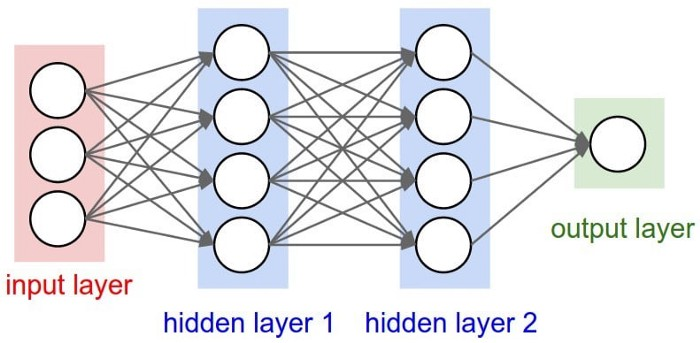
\includegraphics[draft=true, width=0.8\textwidth]{Chapter_introduction/ann}
    \else
        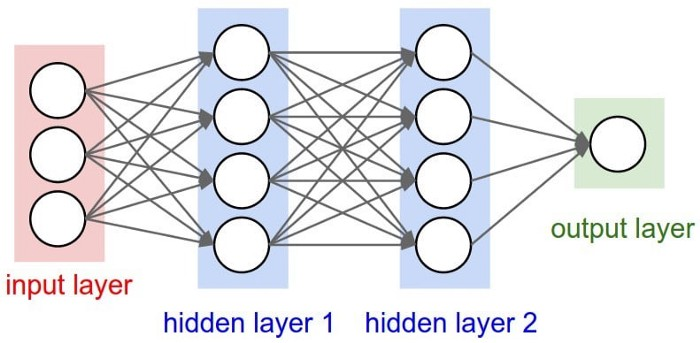
\includegraphics[width=0.8\textwidth]{Chapter_introduction/ann}
    \fi
    \caption{%
        General architecture of an artificial neural network.
        The input layer is processed by two fully-connected hidden layers with the four neurons.
        The model outputs a scalar number from a single neuron.
        Figure taken from https://medium.com/towards-artificial-intelligence/artificial-neural-network-ship-crew-size-prediction-model-c04017c7b6fa.
    }
    \label{fig:ann}
\end{figure}

Why is layer stacking so effective? Applying multiple linear functions in series, results in a linear function. Therefore, one might think that there is no added benefit to stacking layers. However, the power of deep ANNs comes not from their ability to learn linear functions, but from their ability to learn non-linear functions. To achieve non-linearity, non-linear activation functions are applied to the output of each neuron. The sigmoid (logistic) function
\[
\sigma(x) = \frac{1}{1+e^{-x}}
\]
has long been the workhorse of ANNs. Sigmoid neurons, however, suffer from the vanishing gradient problem, which is caused by the difficulty of calculating gradients of large positive, or negative, values. More recently, the rectified linear unit (ReLU)
\[
\text{ReLU}(x) = \max(0,x)
\]
and its variants mitigate this problem and perform better than sigmoid activations in deeper networks. ReLU also has the benefit of being cheap to compute.

\subsubsection{Learning}

In a feedforward ANN, information flows forward through the network, through the hidden layers, to produce the output (\ref{fig:ann}). ANNs frame the learning process as an optimisation problem, where an objective function is optimised. Typically the objective is to minimise the loss between the output and the ground truth. For example, in supervised machine learning, the difference between the predicted class probabilities and the ground truth class assignments is minimised.

Objective functions are optimised using gradient descent through a loss landscape. The topology of this landscape is dependent on the model's parameters. During the optimisation process, the model descends through the landscape until it reaches a minimum loss. To do so, the model needs to know the direction (gradient) to travel in to reduce its loss. The gradient of the objective function is computed by back-propagating the loss, backwards through the network \cite{Rumelhart1986}. An optimiser algorithm uses the gradient to update the model's parameters so that the loss of the model is reduced.

So far, we have only dealt with ideal cases where the model's loss always decreases. Learning is made tricky by the non-convex nature of many loss landscapes. In these, local minima, local maxima and saddle points are present where the gradient is $0$. Therefore, these points provide no information about which direction to travel to reach the global minimum.

The partial derivative $\frac{\partial}{\partial \mathbf{x}_i}f(\mathbf{x})$ of a function $f(\mathbf{x})$ gives the direction of the function w.r.t. $\mathbf{x}_i$. By extension, the gradient of a vector $\nabla_\mathbf{x}f(\mathbf{x})$ is a vector containing containing all of the partial derivatives $\mathbf{x}_i$. ANNs use back-propagation to calculate gradients using the chain rule of differentiation.

Classically, ANNs have used the stochastic gradient descent (SGD) optimiser. Calculating the gradient using all training data is expensive, so SGD gets round this by estimating the gradient using a small sample of training examples. SGD introduces the concept of the learning rate $\epsilon$ that is multiplied with the estimate of the gradient $\hat{g}$ to update the parameters $\theta = \theta - \epsilon\hat{g}$. The learning rate can be used to limit large updates to $\theta$, which could occur for certain samples of training examples.

Optimisation of the objective function can become stuck at local minima and saddle points with SGD, which produces inferior models and increases training time. Contemporary optimisers use adaptive learning rates and momentum to train models rapidly by finding the correct direction to move in, whilst not getting stuck in local minima. Momentum encourages models to continue moving in the direction of past gradients, with an exponentially decaying impact. Adaptive learning rates use separate learning rates for parameters that are scaled according to their previous values. One such optimiser that combines both concepts, Adam \cite{Kingma2014}, is particularly popular in the community.

\subsubsection{Regularisation}

Whilst it is easy to train a neural network to perform well on the training data, it can be hard to get good performance on unseen testing data. Regularisation can be applied to encourage models to learn general patterns and to not overfit on the training data. Overfitting is typically monitored on a validation set that is disjoint from the training and testing sets. A simple way to prevent overfitting is to monitor the objective function applied to the validation set. Training is stopped once the loss begins to increase on the validation set, due to overfitting on the training set.

Classical regularisation penalties, such as L1 and L2 loss can be added to loss functions. However, a popular, simple and cheap method of regularisation is dropout \cite{Srivastava2014}. During training, neurons are dropped out at random with probability $1-\rho$. Dropout is not applied at test time, so to ensure inputs are similar between training and testing, during training the activations of retained neurons are scaled by $\frac{1}{\rho}$.

Now we know how models can be trained, we next focus on different types of ANN architectures.

\subsection{Encoder-decoders}
\label{sec:intro-encoder-decoder}

Encoder-decoders are a general framework used by embedding methods \cite{Hamilton2017}. In encoder-decoders, the encoder first transforms the input data to low-dimensional embeddings, followed by reconstruction of the original data by the decoder, using only the embeddings (\ref{fig:ae})
\[
\text{DEC}(\text{ENC}(\mathbf{X})) = \mathbf{X'} \approx \mathbf{X}
\]
$\text{ENC}$ and $\text{DEC}$ are optimised such that $\text{ENC}(\mathbf{X}) = \mathbf{h}$ and $\text{DEC}(\mathbf{h}) = \mathbf{X'}$. Transitively, if the original data can be reconstructed by the encoder-decoder model, then the embeddings must contain all salient information in the original data. As such, the embeddings can be used as learnt features to train machine learning models.

\begin{figure}[!hbt]
    \centering
    \ifredact
        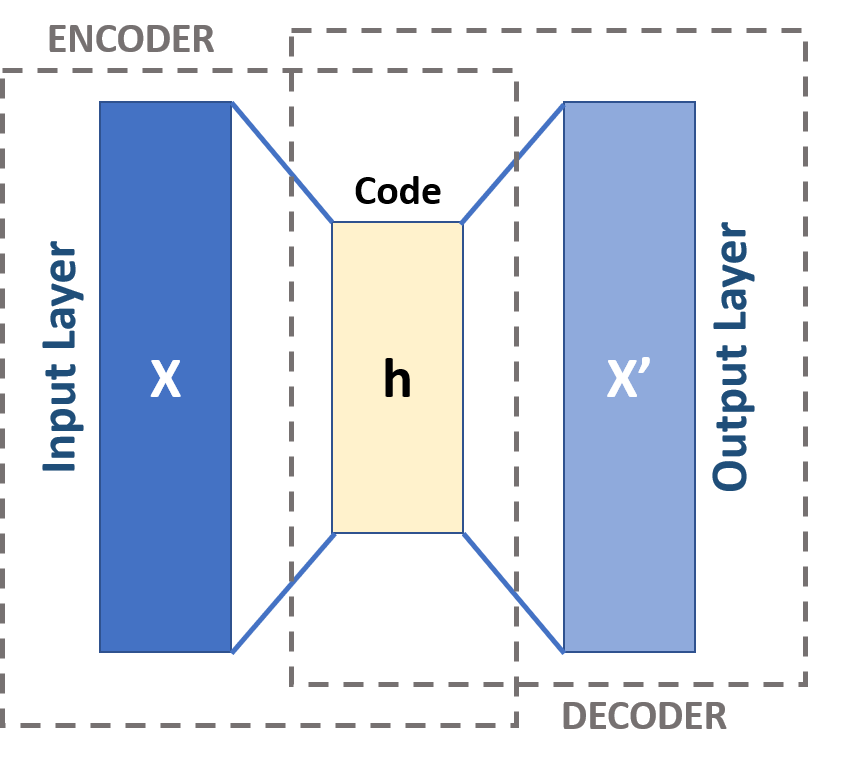
\includegraphics[draft=true]{Chapter_introduction/ae}
    \else
        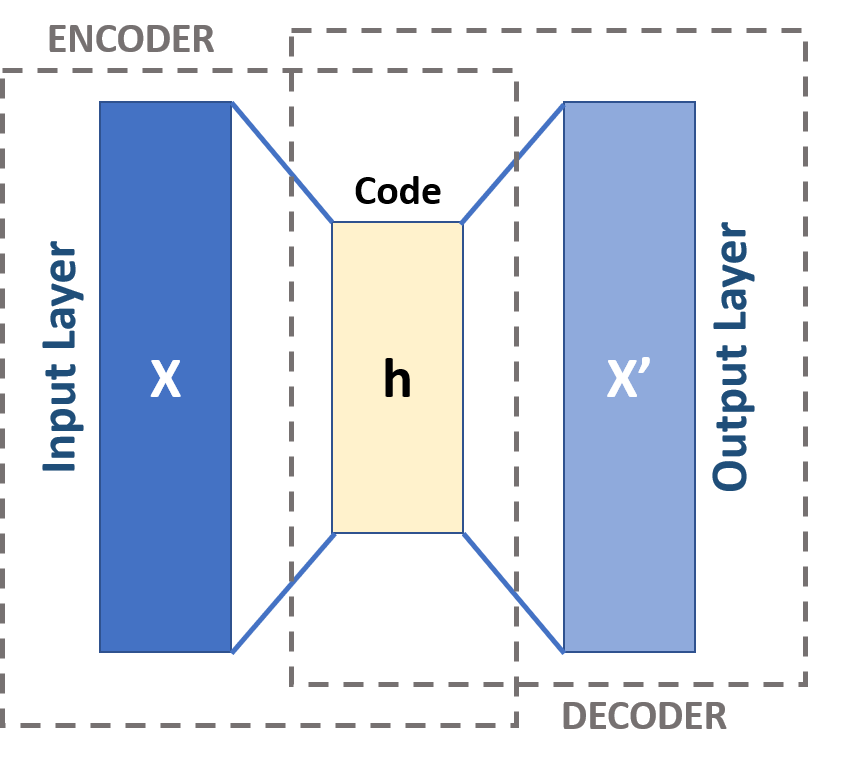
\includegraphics{Chapter_introduction/ae}
    \fi
    \caption{%
        Architecture of a general encoder-decoder model.
        Figure taken from https://en.wikipedia.org/wiki/Autoencoder.
    }
    \label{fig:ae}
\end{figure}

The encoder and decoder functions are learnt in an unsupervised way from the data using an optimisation process. In order to do this, a loss function must be defined to measure the difference between the original data and its reconstruction from the embeddings. The encoder and decoder functions and then optimised to minimise the reconstruction loss, and, concomitantly, the embeddings are improved.

Encoder-decoder models can be divided into direct-encoding and generalised methods \cite{Hamilton2017}. Direct-encoding methods learn an embedding matrix $\mathbf{Z}$, where embeddings are simply
\[
\text{ENC}(v_i) = \mathbf{Zv}_i
\]
where $\mathbf{v}_i$ is a one-hot indicator vector corresponding to element $v_i$.

We will encounter many applications of encoder-decoder neural networks in \ref{sec:intro-ml-application}. In the next section, we explain one general application of the encoder-decoder framework to ANNs in the form of autoencoders.

\subsection{Autoencoders}

Autoencoders are unsupervised neural network encoder-decoder models that attempt to reconstruct their input $\mathbf{X}$ via a hidden representation $\mathbf{h}$ (\ref{fig:ae}). Typically, autoencoders are used for unsupervised feature learning, where $\mathbf{h}$ are a small number of informative features, where $|\mathbf{h}| << |\mathbf{X}|$, that are automatically extracted from $\mathbf{X}$. This process is also referred to as learning an embedding of $\mathbf{X}$. The features learnt in $\mathbf{h}$ can be used for supervised machine learning, distance estimation, dimensionality reduction, denoising data and modelling latent variables. We focus on applications of autoencoders in \ref{sec:intro-encoder-decoder}.

A typical autoencoder architecture might look like
\[
\mathbf{X} \rightarrow \text{ENC} \rightarrow \mathbf{h} \rightarrow \text{DEC} \rightarrow \mathbf{X}'.
\]
Here, an encoder function generates the hidden representation $\text{ENC}(\mathbf{X}) = h$ and a decoder function decodes $\mathbf{h}$ to reconstruct $\mathbf{X}$ as closely as possible $\text{DEC}(\mathbf{h}) = \mathbf{X}'$.

Autoencoders are trained to minimise the loss between $\mathbf{X}$ and $\mathbf{X}'$, $L(\mathbf{X}', \mathbf{X})$. The simplest way for the autoencoder to have a small loss is to learn the identity function $\mathbf{X} = \text{ENC}(\mathbf{X}) = \mathbf{h} = \text{DEC}(\mathbf{h}) = \mathbf{X}'$. However, as we shall see, this defeats the purpose of why one would want to use an autoencoder in the first place.

Restrictions are placed on the autoencoder so that the encoder function must actually learn from $\mathbf{X}$.
The autoencoder is prevented from being able to reconstruct $\mathbf{X}$ perfectly and is forced to prioritise learning useful features in $\mathbf{h}$. As such, overfitting is not a problem when training autoencoders.
Undercomplete autoencoders employ the simplest restriction, where $\mathbf{h}$ is made to have fewer dimensions than $\mathbf{X}$. 
Interestingly, when the encoder and decoder functions are linear and $L$ is the mean squared error, an undercomplete autoencoder recapitulates PCA.
With nonlinear encoder and decoder functions, autoencoders are able to learn nonlinear decompositions of $\mathbf{X}$ that are more powerful than PCA.
In addition to restricting the number of neurons in $\mathbf{h}$, other restrictions can be applied, such as sparsity or noise.
Sparse autoencoders apply an L1 sparsity penalty $\Omega(\mathbf{h})$ to the hidden layer, which encourages only important neurons in the hidden layer to fire.
In denoising autoencoders, random noise is applied to the input $\mathbf{\tilde{X}}$ and the autoencoder is trained to minimise $L(\mathbf{\tilde{X}}', \mathbf{X})$.
The autoencoder must learn to undo the noise and thus learn the true structure of $\mathbf{X}$.

Like many machine learning methods, autoencoders learn to map inputs to a low-dimensional manifold. Variational autoencoders train latent variables to learn the structure of this manifold. These latent variables can be used to generate synthetic examples at some position on the manifold, and smoothly interpolate synthetic examples across the surface of the manifold.

\subsection{Convolutional neural networks}

Convolutional neural networks (CNNs) were introduced by Yann LeCun in his seminal 1989 work to recognise handwritten characters \cite{LeCun1989}. CNNs are ideally suited to grid-like data, such as sequences ($1$D) or images ($2$D). As the name implies, CNNs are ANNs that apply convolutional operations, as opposed to matrix multiplication, in at least one of their layers. CNNs gained notoriety when Alex Krizhevsky won the ImageNet object recognition challenge in 2012 using a deep CNN \cite{Krizhevsky2012}.

A convolutional layer is composed of a set of small filters that recognise features in the input. Each filter is only able to recognise a single feature, however this feature can be recognised at any position in the input. For example, convolution may be applied to a $5\times 5$ window of pixels in an image. The architecture of a typical convolutional layer is often
\[
\text{Conv} \rightarrow \text{Pooling} \rightarrow \text{Activation}
\]
(pooling is explained below).

Convolutional layers provide three benefits to traditional neural network architectures \cite{Goodfellow2016}: parameter sharing, sparse interactions and translation equivariance. Parameter sharing occurs within a single filter, such that the filter's weights are applied to each portion of the input, instead of learning a separate weight for every coordinate. As such, a convolutional layer has a set of sparse interactions between its input and output governed by the size of the filter. Sparse interactions give rise to the receptive field of a convolutional layer. If a feature is recognised by a filter, it will be represented in its output. This output is equivariant to translation within the input: a feature occurring early in the input will be represented early in the output. If this same pattern occurred late in the input, its representation would be exactly the same but translated later in the output. It should be noted that convolution is not equivariant to scaling or rotational transformations.

For a convolutional layer with kernel of width $k$, the width of the output is shrunk by $k-1$. The extent of downsampling is controlled by the depth of the convolutional layers and the widths of their kernels. To prevent shrinkage, zero padding can be applied before convolution is applied by subsequent convolutional layers. In some cases, downsampling may be desirable to increase the computational efficiency of the model. Downsampling can also be achieved by applying convolution with a stride to skip some positions of the filter.

Pooling is applied to the output of a convolutional layer and calculates a statistic that summarises the outputs in a window. One type, max pooling, calculates the maximum value within a window of $n$ inputs. For example, $4$-max pooling of $\begin{bmatrix}0.4, 0.7, 0.3, 0.5\end{bmatrix}$ produces $0.7$. Pooling helps to make features invariant to translation, that is small changes in the input do not change the output. This property is desirable if the task is to recognise features in the input, regardless of their position. To improve a model's computational efficiency by reducing the number of parameters, pooling is often used to downsample an output by using fewer pooling units than output units.

\subsection{Recurrent neural networks}

Recurrent neural networks (RNNs) are a class of neural network that can be used to process sequences through repeated application of the network to each time step in the sequence. Like CNNs, RNNs employ parameter sharing, whereby the same parameters are used to process each time step. RNNs have been successfully applied to text, audio and sensor data. Whilst an in-depth introduction to RNNs is beyond the scope of this chapter, we introduce their salient details and limitations here.

Whilst RNNs are synonymous with sequence modelling \cite{Bai2018}, they do posses some significant drawbacks, namely sequential dependencies, vanishing/exploding gradients and poor memory, that we outline below. For these reasons, RNNs have fallen out of favour at the big tech companies, in favour of convolutional architectures, such as attention-based networks \cite{Xu2015,Elbayad2018}. A very recent class of CNN, temporal CNNs \cite{Bai2018}, are optimised for modelling sequences and outperform RNNs on a wide range of sequence modelling benchmarks.

\begin{itemize}
    \item \textbf{Sequential dependencies}

    RNNs are applied sequentially to input sequences $x$ of length $\tau$ from time point $1$ to $\tau$. The output of an RNN at time $t$ is a function of $x^{(t)}$ and all previous time steps $x^{(1)},...,x^{(t^{-1})}$. Note that time steps need not actually correspond to \emph{time}, but can instead correspond to \emph{position} in the sequence. RNNs can even be used to predict future states of a sequence at times $t > \tau$, as is used in next word text prediction. Despite the impressive results that have been obtained using RNNs, they can be challenging to train, due to the dependency of processing all time steps $1,...,t^{-1}$ before processing $t$.

    \item \textbf{Vanishing/exploding gradients}

    To process a sequence, RNNs build a very deep computational graph, through which it is often difficult to calculate the gradient. This can lead to the problem of vanishing, or exploding, gradients during training, which make it difficult to know which direction to update a model's parameters---and in the case of exploding gradients can make parameters fluctuate wildly during training.

    \item \textbf{Poor memory}

    RNNs can learn dependencies between positions in sequences. However, learning long-term dependencies is challenging, due to the weights of dependencies decreasing in size exponentially with their distance. This means that short-term dependencies with larger weights will tend to dominate the learning process and that it will take a very long time to learn long-term dependencies. A vanilla RNN has been shown to struggle to learn dependencies in sequences of length $20$ \cite{Bengio1994}. Variants of the RNN, such as the long short-term memory (LSTM) network \cite{Hochreiter1997} claim to increase this limit to \num{1000} time steps, however, in practice LSTMs are only able to handle sequences up to $250$ in length.
\end{itemize}

\subsection{Random forests}
\label{sec:intro-rf}

Decision trees are binary trees that segregate data into groups. Items begin at the root node, and traverse the tree towards the terminal nodes, with each internal decision node’s predicate determining the which node the item will visit next. Because the global optimum partitioning of the data is NP-complete \cite{hyafil1976constructing}, the classification and regression trees (CART) algorithm uses a recursive greedy procedure to grow decision trees.

In the training phase, trees are grown by splitting the data according to the predicate that minimises the error at each internal node. A cost function is used to decide if a node is worth splitting, otherwise it will become a terminal node. Cost functions typically take into account the following criteria. If the node is split:
\begin{itemize}
    \item Will the tree have reached the maximum depth?
    \item Will there be too few samples in either of the two nodes?
    \item Will the purity of the node be increased above some threshold?
\end{itemize}
Once a tree has been grown to its full length, it can pruned to prevent overfitting by reducing the number of terminal nodes without increasing the prediction error substantially. 

In the prediction phase, each example begins at the root node and follows a path along the tree’s branches—according to its feature values—until it reaches a terminal node. The label associated with the leaf node is assigned.

Whilst the CART algorithm is useful, it does have several problems. Firstly, the data may not be partitioned optimally, so the global minimum error will not be achieved. Secondly, CARTs are sensitive to the training data, and small changes to the training data can result in the growth of very different trees. Random forests (RFs) attempt to mitigate these two problems and help to reduce the variance of the model.

RFs are ensembles of CARTs. RFs use a technique called bootstrap aggregating, or `bagging', to reduce the variance of the model. Each decision tree in an RF is trained on random subsets of the features and examples, from which bootstrap samples are drawn. Bootstraping is a resampling method that can be used to estimate a sampling distribution. Let $X$ be some sample data drawn from an unknown distribution $S$. $S$ can be estimated by $n$ bootstrap samples, $b$. $b_i$ is generated by sampling $|X|$ items from $X$ with replacement. To increase the differences between each tree in an RF, a random subset of features can also be selected to be included in the training data for each tree. The proportion of samples and features to be included in each subset are hyperparameters, optimised during training.

The number of trees in the forest is not a hyperparameter that should be optimised \cite{Probst2018}. Generally, the largest number of trees that can be trained appropriately on the available resources should be selected. Training and prediction of RFs is embarrassingly parallel because each tree is independent. However, for prediction, the added overhead associated with splitting the task across multiple processors does not typically outweigh applying each tree in serial on a single processor.

In the prediction phase, each tree in the RF has an equal vote. In the classification paradigm, RFs use the majority vote to predict the class of an example. In RF regression, the probability that an example is from some class is the proportion of trees that predicted that class

\subsection{Support vector machines}
\label{sec:intro-svm}

Support vector machines (SVMs) are supervised machine learning models that classify data into one of two classes \cite{Cristianini2004}.
During training, the SVM learns a hyperplane in the training data space that maximises the separation between the data points from the two classes.
In the ideal case, data points from each class will be well separated, with a maximum margin between the hyperplane and the nearest data points from each class.
The data points that lie on the margin on either side of the hyperplane are known as the support vectors.
We discuss applications of SVMs in \ref{sec:intro-graph-kernel,sec:intro-deepnf}.

SVMs are inherently linear classifiers, however SVMs are able to perform more complex, non-linear classification by use of the kernel trick.
Instead of performing classification in the original data space, SVMs first map the data to a high-dimensional space, in which the two classes are more likely to be separable by a hyperplane.
To do this, a kernel function is applied to the data, which calculates dot products between data points in a high-dimensional space, without actually mapping the data points to the high-dimensional space.
Implicitly, kernel functions allow SVMs to produce a curved decision plane in the original feature space, which is actually a straight hyperplane in the kernel space.
Kernel functions should be selected according to the particular task at hand, but one popular and flexible kernel, that produces curved decision boundaries, is the radial basis function kernel.

Real-world data is rarely ideal, so SVMs must make certain trade-offs when optimising the separating hyperplane between how important misclassifications and true classifications are.
To do this, SVMs have a hyperparameter, the soft-margin penalty $C$, that controls the penalty applied to errors.
Lower values of $C$ produce boundaries with larger margins, which increase the risk of misclassifications but reduce the chance of overfitting.
On the other hand, larger values of $C$ produce decision boundaries with a small margin between the two classes, at the risk of overfitting on the training data.
The hyperparameter should be optimised during model training, in addition to other hyperparameters that are specific to particular kernel functions.
For example, the radial basis function kernel has the $\gamma$ hyperparameter that controls the influence of the data points on the hyperplane, with high values increasing the locality of the influence and low values extending the range of influence.

\section{Modern applications of machine learning to protein data}
\label{sec:intro-ml-application}

Since beginning my PhD, bioinformatics has witnessed an explosion of machine learning research based on ANNs---or `deep learning' as it is sometimes, and often incorrectly, referred to. These topics have been reviewed in many publications, but we believe, subjectively, that the following reviews are best \cite{Angermueller2016,Ching2017,Min2016,LeCun2015,Baldi2018,Schmidhuber2015,Goodfellow2016,Wainberg2018}. The ensuing explosion has resulted in ANNs being used so widely in bioinformatics that it would be beyond the scope of any single piece of work to cover all topics. Instead, we focus here on the more relevant advances and applications to the task of protein function prediction and the related task of protein family prediction. Specifically, we focus on methods that allow machine learning to be applied directly to network and sequence data, without the need for feature engineering. These methods feel almost like magic and would have been inconceivable just a decade ago. Astute readers may notice some commonalities between the names of methods that we introduce here\ldots{}

The timing of the advances in biological data generation and ANNs have coincided at an ideal time. High-throughput methods now generate unprecedented volumes of experimental data, that classical bioinformatics techniques struggle to process. ANNs are powerful statistical models that require large amounts of data and computational power to train. ANNs have already been proven to be a valuable tool in the bioinformatics toolbox. We conclude that we have set out along a path in which ANNs will permanently transform bioinformatics.

\subsection{Protein networks}

Graphs are ubiquitous data structures. Graphs have many important applications, including machine learning on graphs. For example, recommendation engines---such as those used at Netflix, Spotify and Amazon---predict shows, music and products for users. Here, we introduce a number of techniques that allow machine learning to be applied to graphs. All of the methods involve calculating a node embedding in the graph. Comprehensive reviews of the latest advances in this topic can be found in references \cite{Hamilton2017,Cai2017}.


\subsubsection{Graph embeddings}
\label{sec:intro-graph-embeddings}

Embedding methods learn representations of nodes that encode structural information about the graph \cite{Hamilton2017}. Embeddings are vectors that represent a set of latent features that are automatically learnt from the graph. The goal is to optimise the embedding, such that relationships in the embedding space recapitualate relationships in the graph space. Graph embeddings have been used previously for protein function prediction \cite{Cho2016,Gligorijevic2018}.

The crucial advance of graph embedding methods is that the function that maps nodes to the embedding space is learnt from the data in an unsupervised way. Graph embedding methods are not domain-specific, so they can be applied to any graph.

Low-dimensional embeddings tend to be learnt, where on the order of $10^2-10^3$ latent dimensions are used. These embeddings are small enough such that they can be used to train off the shelf machine learning models. Alternatively embeddings can be used to calculate distances between nodes---in terms of the differences in their network contexts---with applications in clustering.

We encountered the encoder-decoder framework in \ref{sec:intro-encoder-decoder}. Many graph embedding methods are based on encoder-decoder models. The encoder first maps nodes to low-dimensional embeddings, followed by reconstruction of the original data by the decoder, using only the embeddings. Later, we introduce Mashup \cite{Cho2016}, node2vec \cite{Grover2016} and DeepWalk \cite{Perozzi2014} as examples of direct-encoding methods. This approach has a number of drawbacks, however. Firstly, no parameters are shared in the model and each node's embedding vector is learnt independently. Consequently, models are $\mathcal{O}(|V|)$. Parameter-sharing is a powerful regularisation approach. Secondly, models are static and embeddings can only be generated for nodes available at training time. This is limiting for temporal graphs that change over time and large graphs that cannot be stored in memory. Generalised methods, on the other hand, overcome these limitations by learning more complex encoder functions that share parameters and can be applied to nodes that were not available at training time. Autoencoders are a type of generalised encoder-decoder model, implemented using an unsupervised neural network. Below, we introduce deepNF \cite{Gligorijevic2018} as an example of a generalised encoder-decoder method.

\subsubsection{deepNF}
\label{sec:intro-deepnf}

deepNF \cite{Gligorijevic2018} learns a set of highly informative features, by embedding proteins in a low-dimensional latent space that represents the context of each protein in a protein-interaction network. Conceptually, the multimodal deep autoencoder compresses large volumes of orthogonal information, encoded in multiple types of edges, into a small number of features. Although deepNF was devised for protein-interaction networks, the method is entirely flexible and can be applied to any network that contains multiple, orthogonal types of edges. deepNF was inspired by other (non-biological) approaches to applying deep learning to graphs, including Deep Neural Graph Representations \cite{Cao2016a} and Structural Deep Network Embeddings \cite{Wang2016}.

More formally, deepNF takes a multigraph $G$ with $n$ nodes and learns an embedding that represents the context of each node in this graph. Given $k$ different types of edges in $G$, an autoencoder is used to learn an encoder function that maps the adjacency matrix of $G$ to a low $l$-dimensional embedding space that represents the context of each node across the $k$ edge types. The encoder function is unary, embeddings are generated for each node. An alternative view of deepNF is that $k$ input networks, each with $n$ nodes, are used as input to a multimodal deep autoencoder (\ref{fig:deepNF}). Overall, the autoencoder maps an $[n \times n \times k]$ multigraph adjacency matrix to an $[n \times l]$ embedding matrix, where $l << n$ for any reasonably sized network.

\begin{figure}[!hbt]
    \centering
    \ifredact
        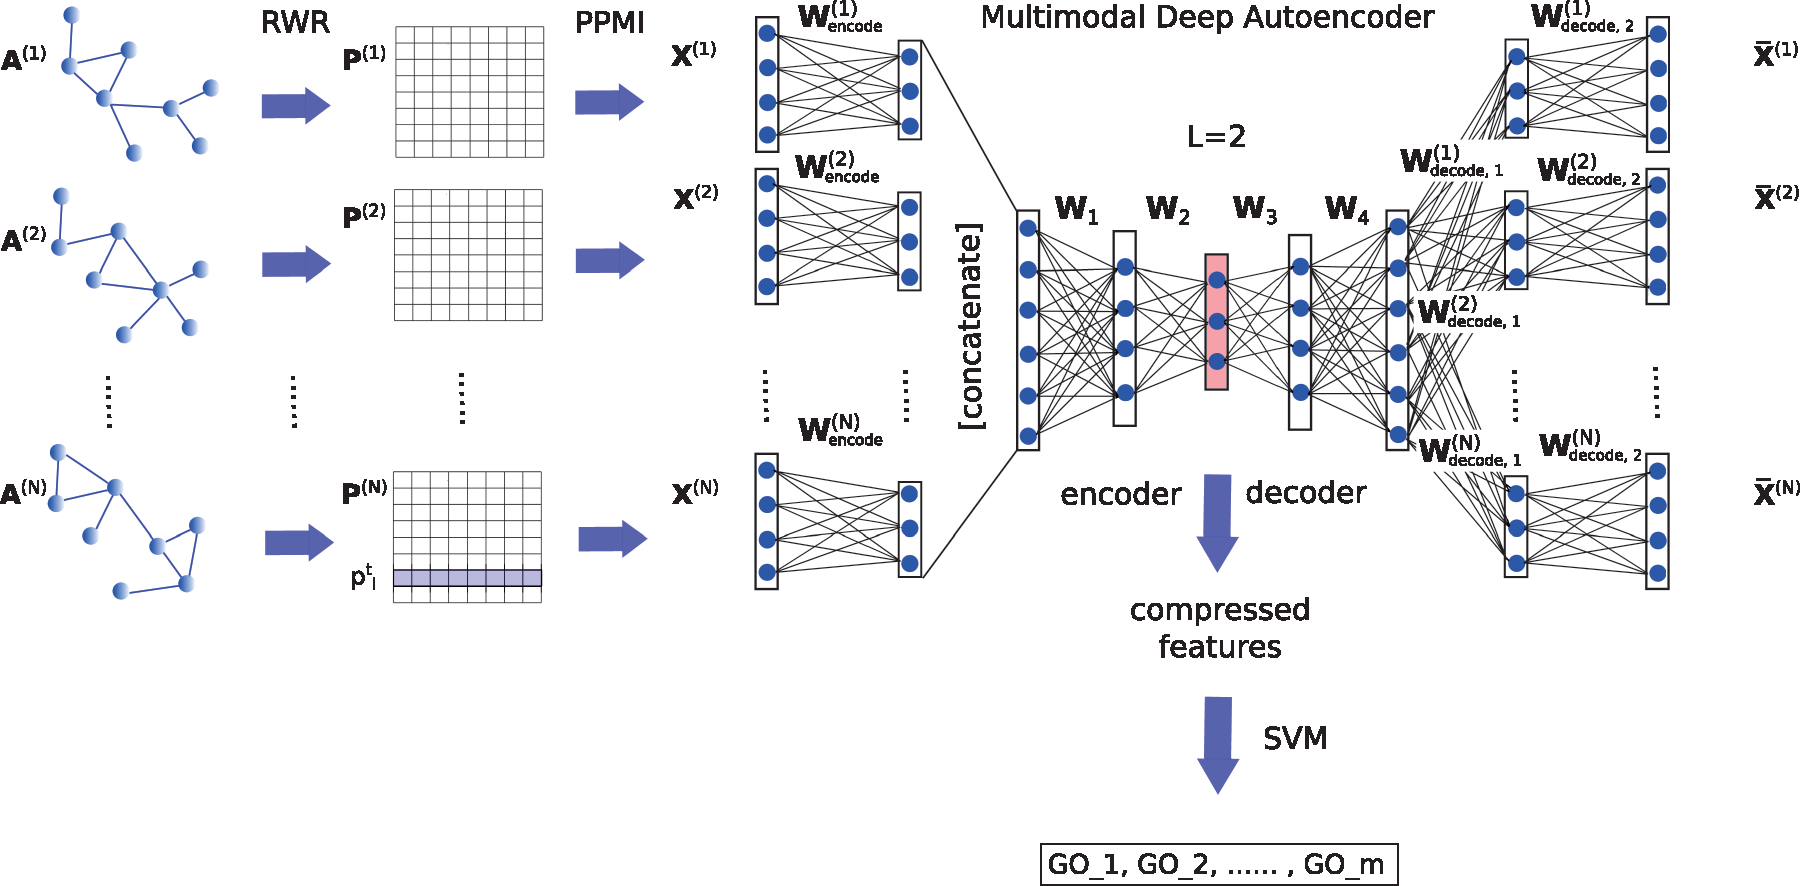
\includegraphics[draft=true, width=\textwidth, trim={0 -1cm 0 -1cm}, clip=true]{Chapter_network_fusion/deepnf_overview}
    \else
        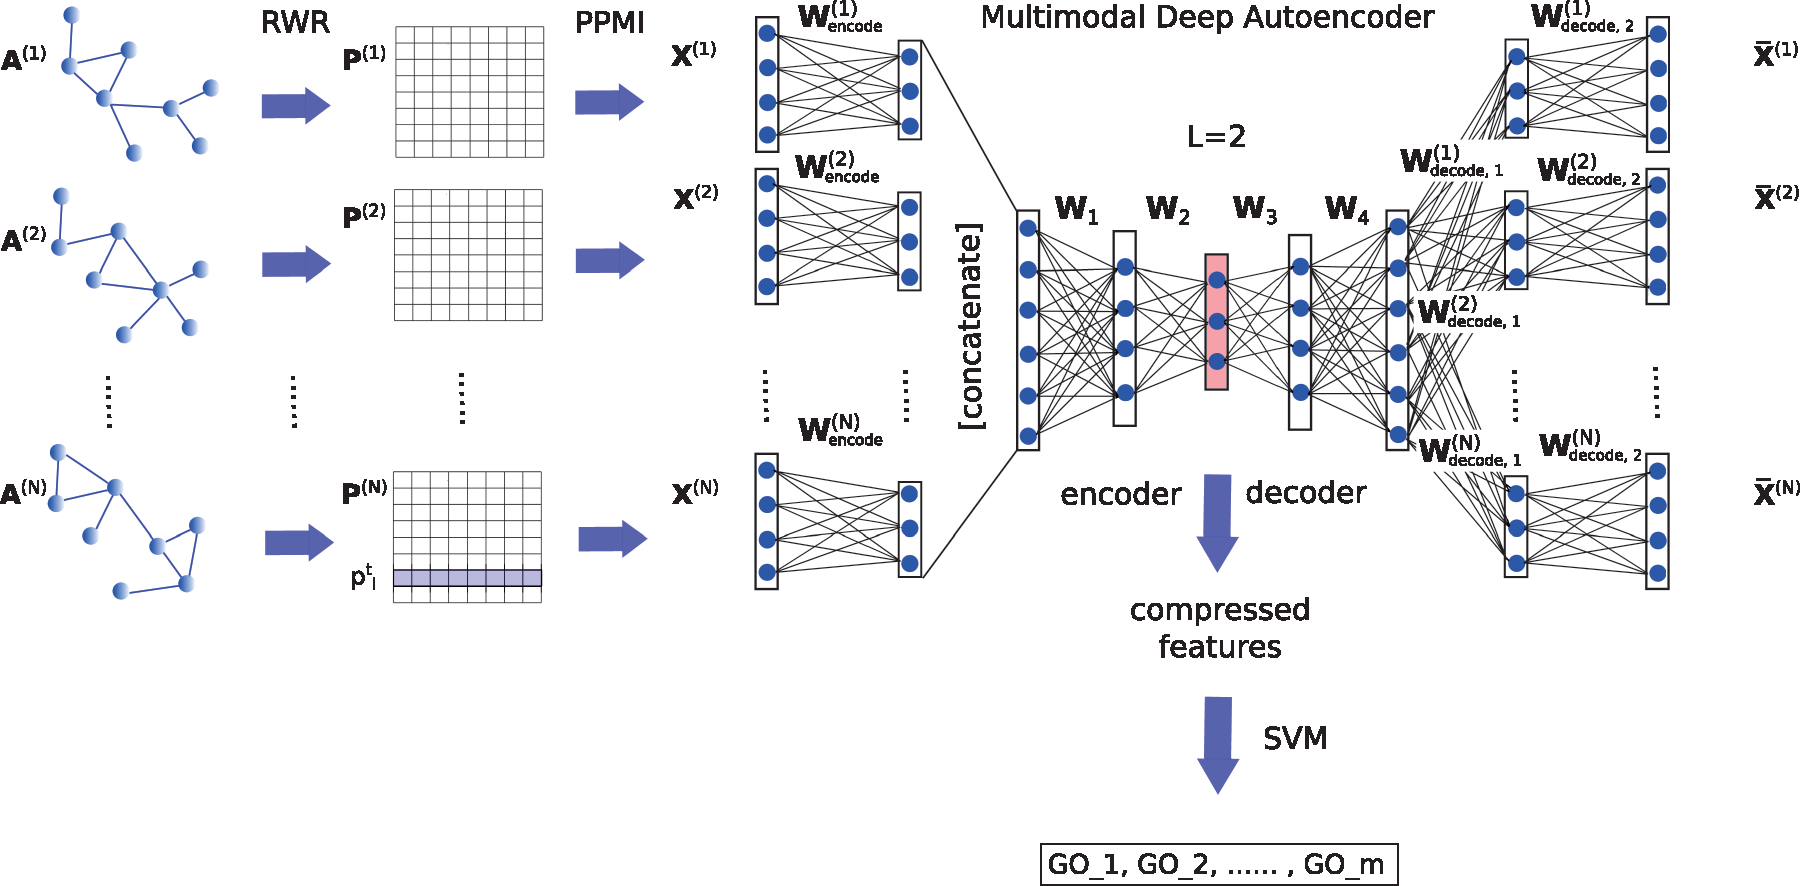
\includegraphics[width=\textwidth, trim={0 -1cm 0 -1cm}, clip=true]{Chapter_network_fusion/deepnf_overview}
    \fi
    \caption{%
        deepNF overview.
        Figure taken from \cite{Gligorijevic2018}.
    }
    \label{fig:deepNF}
\end{figure}

Random walks with restart are applied to the adjacency matrices to calculate a node transition probability matrix. Local and medium-range topologies of the graphs are explored by the random walks. This, in turn, reduces the sparsity of the original adjacency matrix. The pointwise mutual information is then calculated that two nodes occur on the same random walk.

SVMs were trained to predict protein functions using the one-vs-rest multiclass strategy. Radial-basis function kernels were precalculated and cached to speed up training time. Terms were split into three levels according to how many proteins each term is annotated to. As one might expect, more common functions that are annotated to $101-300$ proteins were predicted better than rarer functions annotated to $11-30$ proteins.

deepNF, Deep Neural Graph Representations and Structural Deep Network Embeddings all suffer a number of limitations. Firstly, all require that the input dimension to the autoencoder is $|V|$. In the case of deepNF, the input is even larger, at $k|V|$ for $k$ edge types. Therefore, these methods cannot be applied to large networks with $> 10^5 - 10^6$ nodes, depending on memory resources. Secondly, models are fixed to the number of nodes in $V$ at training time. However, new embeddings can be generated if the original adjacency matrix is rewired, for example under different developmental stages, cellular stresses or other changes in proteome regulation.

We use deepNF extensively in \ref{chapter:network-fusion}. deepNF took much inspiration from another graph embedding method, Mashup \cite{Cho2016}, which we introduce in the next section.

\subsubsection{Mashup}

Mashup \cite{Cho2016} is a similar method to deepNF, in that it learns a low-dimensional embedding of nodes across multiple input networks. Like deepNF, Mashup was developed for protein networks, but the method is not domain-specific and can be applied to model any multigraph problems. However, unlike deepNF, Mashup is a direct-encoding method, cannot be generalised to new nodes and does not share parameters between nodes.

Mashup first calculates a node transition probability matrix using random walks with restart. Low-dimensional embeddings are then calculated by applying a novel dimensionality reduction method. Networks are high-dimensional, incomplete and noisy. We wish to transform the original matrix into a low-dimensional matrix that explains the variance of the original matrix, similar to PCA. Mashup achieves such a dimensionality reduction by framing the process as an optimisation problem. Each node $i$ is represented using two vectors: $x_i$ for features of the node and $w_i$ that captures the context of the node in the topology of the network. (If $x_i$ and $w_j$ are close in direction and have large inner product, then node $j$ will be visited often on random walks beginning at node $i$.) If these vectors $x$ and $w$ do indeed capture topological features of the network, then they can be used to identify similar nodes in the network. Mashup optimises the $x$ and $w$ vectors by minimising the Kullback--Leibler divergence between the observed transition probabilities $s$ and the predicted probabilities $\hat{s}$. This optimisation procedure can be extended to multiple networks, allowing node contexts across heterogenous types of edges to be integrated. The trick is that each of the $k$ networks has its own $w_i^k$ context vector, but node vectors $x_i$ are shared across all networks. The objective function is jointly optimised across all networks. In so doing, latent features of nodes are learnt in an unsupervised way and are captured in the node vectors $x$, which can be used to train machine learning methods.

Node embeddings were successfully applied to a number of biological problems. In all cases, Mashup was benchmarked against a state-of-the-art method and achieved a higher performance.

\begin{itemize}
\item
  Predict protein function, benchmarked against GeneMANIA \cite{Franz2018}.
\item
  Reconstruct Gene Ontology, benchmarked against NeXO \cite{Dutkowski2013}.
\item
  Predict genetic interactions, benchmarked against Ontotype \cite{Yu2016}.
\item
  Predict drug efficacy, benchmarked against a synthetic lethality predictor for cancer drugs \cite{Jerby-Arnon2014}.
\end{itemize}

\subsubsection{node2vec and DeepWalk}

Random walks are also used by two similar methods, node2vec \cite{Grover2016} and DeepWalk \cite{Perozzi2014}, to explore the topology of a network. Both methods learn a pairwise encoder that encodes properties of random walks on the graph between a pair of nodes $i$ and $j$. Consequently, embeddings are stochastic and asymmetric, i.e.~they are direction-specific from $i$ to $j$. These methods frame network embedding as a problem in the style of natural language processing, where nodes are words, the set of random walks is a corpus of text and paths are sentences sampled from the corpus.

DeepWalk is based on a random walk model that uses the edge weights to decide each node-to-node transition. node2vec, on the other hand, implements a more advanced random walk model that is parametric and can be biased to perform more depth-first or bredth-first searches.

node2vec was extended to handle multiple networks, representing different types of edges, in OhmNet \cite{Zitnik2017}. Whilst no parameters were shared, a regularisation penalty was applied that linked the embeddings of a node across each of the $k$ networks.

We focus here on methods that employ random walks on graph nodes. A number of methods exist that are not based on random walks but are conceptually similar to node2vec and DeepWalk, including LINE \cite{Tang2015} and HARP \cite{Chen2018a}.

\subsubsection{Graph kernels}
\label{sec:intro-graph-kernel}

Graph kernels can be calculated by applying a kernel function to all node pairs in the graph \cite{Fouss2012}. The kernel value for each pair of nodes recapitulates the context of these nodes in the graph and the kernel represents the overall topology of the graph. Graph kernels of functional association networks, such as protein-interaction networks, can be used for protein function prediction \cite{Heriche2014,Lehtinen2015}.

Firstly, kernels can be queried directly using a seed set of proteins that are known to have some function \cite{Lehtinen2015}. Under the guilt by association framework, the remaining proteins in the kernel can be ranked by their similarity to the seed set. Highly-ranked proteins are likely to have the function, and vice versa for low-ranked proteins.

Secondly, kernels can be used for data fusion because a combination of kernels is also a kernel \cite{Cristianini2004}. As such, heterogenous information across multiple networks can be fused by combining their graph kernels. This approach was taken by Hériché et al. to fuse a range of human gene and protein association networks, in order to predict novel genes involved in chromatin condensation \cite{Heriche2014}. Nine genes known to be involved in this process were used as seeds to rank the remainder of the genome. An RNAi screen of the $100$ best-ranked genes identified $32$ that caused defective chromatin condensation when knocked down. Hit rates in RNAi screens are notoriously low, so these results correspond to an order of magnitude improvement on the median hit rate in mammalian cells \cite{Sigoillot2011}.

Third and finally, kernels can be used directly in kernel-based machine learning models (\ref{sec:intro-svm}). SVMs are an obvious type of kernel-based model, but many other types of models exist \cite{Cristianini2004}, including kernel partial least squares regression, kernel principal component analysis and kernel Fisher linear discriminant analysis. Often the radial basis function kernel is used in SVMs, but, if desired, tailored kernel functions can be used and the resulting kernel used directly in the SVM. For example, Lehtinen et al. \cite{Lehtinen2015} used a commute time kernel of the STRING \cite{VonMering2005a} network to predict protein function using kernel partial least squares regression. This method outperformed GeneMANIA \cite{Mostafavi2008}, the best performing method at the time.

Principal component analysis is the eigenvalue decomposition of a positive semi-definite covariance matrix. Adjacency matrices are not positive semi-definite, but the Laplacian matrix and graph kernels are. Principal component analysis has also been applied to commute time graph kernels \cite{Saerens2004}. In so doing, spectral clustering \cite{Bach2004} of the principal components therefore has a tangible interpretation in terms of random walks on the graph nodes \cite{Saerens2004}, where clusters are sets of nodes in the graph with high modularity.

\subsection{Protein sequences}

One of the most powerful features of ANNs in computational biology is the ability for models to be applied directly to DNA, RNA and protein sequences \cite{Angermueller2016}. Classical machine learning methods---such as decision trees and support vector machines---require manual feature engineering to extract information from sequences manually. Examples of hand-engineered features include $k$-mer frequencies, torsion angles, presence of secondary structural elements and distance from a protein functional site \cite{Das2020}. Often motif information is not captured \cite{Zhang2020}. ANNs do not require features to be hand-engineered. Instead, models can learn to extract features directly from the data. In the case of biological sequence data, models can detect sequence motifs by learning correlations between positions in the sequence, similar to, but more powerful than, HMMs \cite{Zhang2020,Seo2018}.

Biological sequences are vectors of categorical features from an alphabet $\Sigma$. Neural networks require numerical inputs, so sequences are one-hot encoded. For example the DNA $4$-mer ATCG could be one-hot encoded as:
\[
\begin{bmatrix}
    \text{A} \\
    \text{C} \\
    \text{G} \\
    \text{T}
\end{bmatrix}
\rightarrow
\begin{bmatrix}
    1 & 0 & 0 & 0 \\
    0 & 1 & 0 & 0 \\
    0 & 0 & 1 & 0 \\
    0 & 0 & 0 & 1
\end{bmatrix}
\]
As such, one-hot encoded sequences can be thought of as $[n\times 1]$ images with $\Sigma$ colour channels.

Most ANNs---with the exception of certain convolutional and recurrent architectures---require fixed-width inputs. Autoencoders require fixed-width inputs, so that the model can reconstruct inputs from encodings. Collections of variable-width sequences can be converted into fixed-width inputs by padding one-hot encodings with zeros \cite{Seo2018} or a uniform distribution over $\Sigma$ \cite{Alipanahi2015}.

Studies using genomic sequences tend to divide sequences into shorter, more manageable $600$ bp \cite{Kelley2016} or \num{1000} bp sequences \cite{Quang2016,Zhou2015,Angermueller2017} centred on a region of interest. Protein sequences are much shorter than genomic sequences, so entire protein sequences tend to be used.

One particularly interesting application of ANNs to biological sequences is that of embedding sequences in a low-dimensional latent space. In the same way as graph embeddings introduced in \ref{sec:intro-graph-embeddings}, these embeddings can be used as features to train off the shelf machine learning models. In the next section, we describe how sequence embedding methods work and introduce some of the ways they have been applied to sequence-based prediction problems in bioinformatics.

\subsubsection{Sequence embeddings}
\label{sec:intro-sequence-embeddings}

The field of natural language processing has developed an array of machine learning methods to learn from text. One nascent approach is that of text embedding. These methods embed variable-length sequences into fixed-length, low-dimensional vectors. The first method to implement this approach was word2vec \cite{Mikolov}, which embedded words and phrases. word2vec inspired many other approaches, including doc2vec \cite{Le2014}, for longer sequences of sentences, paragraphs and documents.

Recent natural language processing methods are able to capture information about word order and semantics. Examples include the continuous bag of words model, where a set of context words are used to predict a target word, and the skip-gram model, where a target word is used to predict the context word. Using these methods in embedding methods allows the embedding space to capture information about word order and semantics in the original text space. Thus, `dog' and `cat' will be closer in the embedding space than `dog' and `car', despite differing by only one letter. Word embeddings can be used to answer algebraic questions \cite{Le2014}, such as
\[
\overrightarrow{\text{king}} - \overrightarrow{\text{man}} + \overrightarrow{\text{woman}} = \overrightarrow{\text{queen}}.
\]
Embeddings allow off the shelf machine learning models, that require a fixed number of features, to be trained on any set of sequences. Alternatively, vectors can be directly compared using distance metrics in vector space, such as the cosine distance.

Sequence embeddings can also be used for alignment-free sequence comparison \cite{Ren2018}. Sequence alignment is expensive, particularly when performing pairwise alignments of large sets of sequences. Other alignment-free sequence comparison methods, such as those based on hashing, provide an approximate measure of the similarity between two sequences, without direct comparison of the sequences. These methods represent sequences as a low-dimensional vector by selecting $m$ unique $k$-mers from each sequence. Each $k$-mer is hashed to a number (hash value), which is used to determine whether to select this $k$-mer to represent the sequence. MinHash is one hashing method that represents sequences using the $m$ numerically smallest unique hash values obtained by hashing all $k$-mers in a sequence \cite{Ondov2016,Buhler2001,Luo2019,Steinegger2018}. Sequences can be compared rapidly by calculating an approximate distance as the pairwise Jaccard index,
\[
J(X,Y) = \frac{|X \cap Y|}{|X \cup Y|},
\]
between sets of hash values $X$ and $Y$. Although hashing techniques are incredibly efficient and powerful, sets of $k$-mers do not retain semantic information about the context of $k$-mers in the sequence. The sequence embedding methods that we introduce below are able to represent sequences using a low-dimensional vector that does retain semantic information.

Convolutional architectures have permitted networks to be trained on raw data, such as DNA and protein sequences \cite{Angermueller2016}. Hand-engineered features no longer need to be calculated from sequences; instead, the CNN learns to extract (non-linear) features from sequences automatically. Not only does this save time, but the extracted features are high-quality and lead to greater performance \cite{Angermueller2016}.

ANN text embedding methods are based on the encoder-decoder model that was introduced in \ref{sec:intro-encoder-decoder}. However, whereas network embedding methods use autoencoders to learn embeddings in an unsupervised manner, in sequence embedding, natural language processing methods are used to generate embeddings from unlabelled data. Whilst sequence embedding methods are, overall, unsupervised, the learning objective is posed as a supervised classification problem. One interesting early application of this approach was in Semantic Hashing \cite{Salakhutdinov2009} for document classification, however, here we focus on more recent methods.

\subsubsection{word2vec}

word2vec \cite{Mikolov} takes a corpus of text, composed of words from word set $\mathcal{V}$, and generates $n$-dimensional embeddings for each word. A neural network is constructed, consisting of a $V$-dimensional input layer, where $V = |\mathcal{V}|$, an $N$-dimensional hidden layer and a $V$-dimensional output layer (\ref{fig:word2vec}; we use the notation from this figure in the remainder of this section). The architecture is intentionally shallow to allow it to be trained efficiently on large corpuses, where $V > 10^9$. This architecture is reminiscent of an autoencoder with a single hidden layer, but the training objective is different.

word2vec can be run in two modes: continuous bag of words or skip-gram. We use the continuous bag of words mode as an example. Here, $C$ context words $x_k$ are fed to the network as one-hot $V$-dimensional vectors and are processed by a word matrix $\mathbf{W}$. Neurons in the hidden layer $h$ are trained, using the average of the $C$ context word outputs, to predict the target word $y_j$. Embeddings are processed by the $\mathbf{W}'$ matrix to generate outputs. Outputs are converted to probabilities using the softmax function. The network is optimised by reducing the loss between the target word $y_j$ and the predicted words $y$.

\begin{figure}[!hbt]
    \centering
    \ifredact
        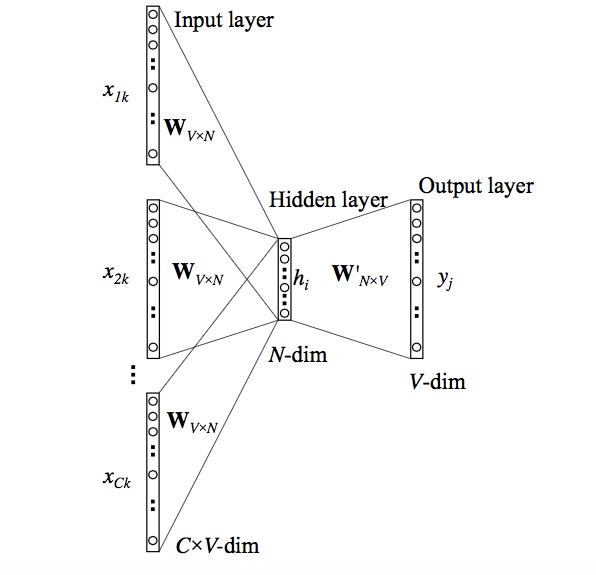
\includegraphics[draft=true]{./Chapter_introduction/word2vec}
    \else
        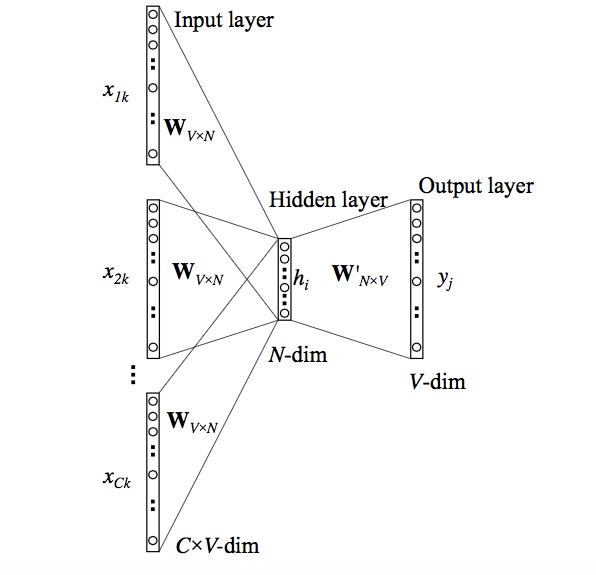
\includegraphics{./Chapter_introduction/word2vec}
    \fi
    \caption{%
        word2vec neural network architecture.
        The continuous bag of words mode is shown.
        Figure taken from http://www.stokastik.in/understanding-word-vectors-and-word2vec/.
    }
    \label{fig:word2vec}
\end{figure}

\subsubsection{doc2vec}

doc2vec \cite{Le2014} is based on word2vec and generates $n$-dimensional embeddings for each paragraph $P$. One-hot $V$-dimensional vectors of words are shared across all paragraphs and are processed by the word weight matrix $\mathbf{W}$ (\ref{fig:doc2vec}). In addition to being trained on context words, models are simultaneously trained on paragraph IDs. The paragraph ID is shared across all contexts of a paragraph and is processed by the paragraph weight matrix $\mathbf{D}$. The paragraph ID can be thought of as an additional word that links the context words to particular paragraphs. Therefore, the model is encouraged to learn the semantics of individual words and how they shape the meaning of the paragraphs they occur in. Each paragraph is mapped to an $N$-dimensional vector and each word is mapped to an $M$-dimensional vector. These vectors are concatenated and used to predict the target word in the same way as word2vec. At each step of the training process, $C$ context words are randomly sampled from $P$ and are used to predict the target word.

\begin{figure}[!hbt]
    \centering
    \ifredact
        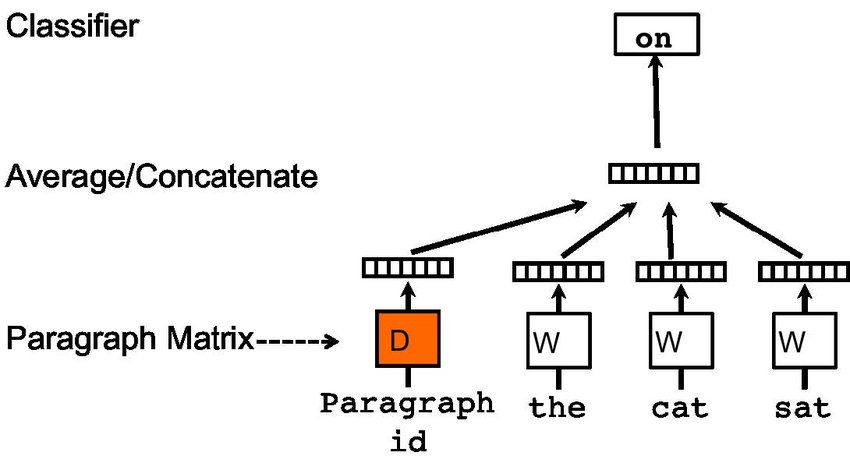
\includegraphics[draft=true]{./Chapter_introduction/doc2vec}
    \else
        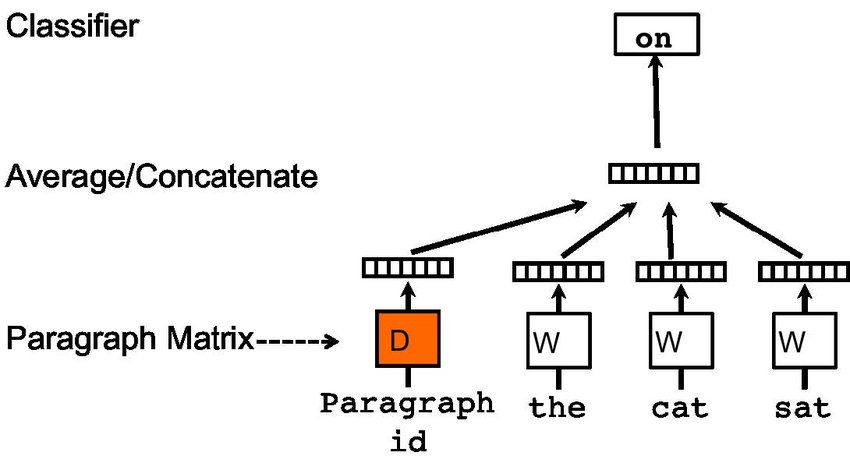
\includegraphics{./Chapter_introduction/doc2vec}
    \fi
    \caption{%
        doc2vec neural network architecture.
        The continuous bag of words mode is shown.
        Figure taken from \cite{Le2014}.
    }
    \label{fig:doc2vec}
\end{figure}

word2vec and doc2vec have been applied in many different ways to biological sequences. Below, we focus on applications to protein sequences. These methods have also been applied to nucleic acid sequences \cite{Asgari2015,Ng2017}.

\subsubsection{BioVec a.k.a. ProtVec}

BioVec a.k.a. ProtVec \cite{Asgari2015} is a sequence embedding method for biological sequences, based on word2vec. Sequences are treated as sentences from a corpus, where $k$-mers of the sequences are treated as words. BioVec embeds sequences according to $k$-mer (word) contexts. Sequences were embedded in a $100$-dimensional space, where the sequence embedding is the summation of embeddings for all $3$-mers in the sequence. BioVec found that $3$-mers were the best length.

The embedding space was shown to encode biophysical properties of the $3$-mers---for example, mass, polarity, hydrophobicity and charge---where $3$-mers with similar biophysical properties had similar embeddings when projected into a $2$-dimensional space using tSNE.

One-vs-rest SVMs were trained on embeddings to predict Pfam families for all of Swiss-Prot, using sequences from a family as positive examples and randomly selected negative examples from all other families. BioVec achieved $93\%$ accuracy on this binary classification task. However, the setup of this experiment is far from how a protein family classifier would be used in real life. Pfam contains \num{7027} families, so the negative set is likely to contain proteins that are significantly different to the positive set---making the binary classification task easy. Ideally, protein family classification needs to be performed using a multiclass prediction strategy, rather than one-vs-rest. Protein family prediction using ANNs is covered in more detail in \ref{sec:intro-protein-families}.

The $100$-dimensional $3$-mer embeddings were used in SDN2GO \cite{Cai2020} to predict GO terms for proteins. SDN2GO is a multimodal ANN model that used network and InterPro protein family information in addition to protein sequences. The BioVec embeddings were processed by two convolutional layers followed by one fully connected layer, before being combined with network and protein family layer outputs to make the final function predictions.

ProtVecX \cite{Asgari2019} is a recent extension to ProtVec, which allows variable-length motifs to be extracted from protein sequences using the byte-pair encoding compression algorithm, which has gained in popularity in the NLP field. The standard ProtVec method is then used to generate embeddings of the extracted motifs.

\subsubsection{seq2vec}

seq2vec \cite{Kimothi2016} is a sequence embedding method for biological sequences, based on doc2vec. seq2vec improves upon BioVec because the overall context of $k$-mers (words) in sequences (documents) are learnt, as well as the semantics of individual $k$-mers. Sequences were embedded using $3$-mers into a $250$-dimensional space.

One-vs-rest SVMs were trained on embeddings to predict Pfam families for all of Swiss-Prot using with $95\%$ accuracy. Multiclass prediction was also tested for seq2vec using a multiclass SVM trained using the one-vs-one strategy, where $n\choose 2$ models are trained to predict all pairs of classes. Here, the accuracy drops to $81\%$ for seq2vec and $77\%$ for BioVec. However, only the largest $25$ Pfam families, which is $< 1\%$ of all families. To be useful for protein family classification in the wild, these methods will need to be able to classify all CATH or Pfam families simultaneously (see \ref{sec:intro-protein-families} for more details on protein family classification). It would be interesting to see how well an MLP performs that is trained to predict a larger number of families simultaneously.

Notably, seq2vec and BioVec were benchmarked against BLAST. Whilst seq2vec consistently performed significantly better than BioVec, BLAST outperformed seq2vec. However, BLAST is one of the most highly engineered pieces of bioinformatics software, so it is natural to expect it to outperform nascent embedding-based methods. At least for now!

\subsubsection{dom2vec}

dom2vec \cite{Melidis2020} is a sequence embedding method for protein sequences that learns to embed protein domains.
dom2vec is based on word2vec \cite{Mikolov} using the continuous bag of words and skip-gram strategies.
Philosophically, BioVec and seq2vec treat amino acids as words and proteins as sentences, whereas, dom2vec treats domains as words and multi-domain architectures as sentences.
InterPro domain MDAs for all UniProt sequences were used as input to a word2vec model
dom2vec was benchmarked against ProtVec \cite{Asgari2015}, which is also based on word2vec, and SeqVec, achieving competitive results.
Extensive benchmarks were conducted for predicting EC classes, molecular function GO terms, InterPro domain hierarchies and SCOPe secondary structure classes.

\subsubsection{SeqVec}

SeqVec \cite{Heinzinger2019} is a sequence embedding method that is not based on word2vec.
Instead, SeqVec is based on ELMo \cite{Peters2018}, an NLP model that predicts the next word in a sequence, given all previous words in the sequence.
ELMo is comprised of a CharCNN, followed by two bi-directional LSTM RNN layers.
The CharCNN learns a context-insensitive vector representation of each character, in this case each amino acid.
The bi-directional LSTM layers take the CharCNN embedding and introduce contextual information.
The forward and backward passes of the LSTM layers are trained independently to avoid the backward and foward passes leaking information to each other.
SeqVec used a $28$ letter alphabet to represent the standard amino acid code, ambiguous residues and special tokens to mark the beginning and end of sequences and padding.
SeqVec generates a \num{1024}D embedding vector from the summation of the \num{1024}D outputs of the three layers at the C-terminus of the sequence.
SeqVec was trained on \num{3e7} protein sequences from UniRef50, containing \num{9e9} residues.
Each residue is a unique sequence context, thus was treated as a separate token in the NLP sense.
SeqVec achieved competitive performance in benchmarking, but had faster run times than the competing methods.

\subsubsection{UniRep}

UniRep \cite{Alley2019} is another LSTM-based sequence embedding method based on an NLP language model.
UniRep and SeqVec were published two months apart, so neither benchmark the other.
The model is trained on protein sequences to predict the next residue in the sequence.
Like SeqVec, an amino acid character embedding is used as input to an LSTM.
Each protein sequence is represented using a \num{1900}D embedding vector.
In order to capture long-range and higher-order dependencies between residues, the embedding was the average of the LSTM layer's hidden state for each amino acid in the protein sequence.
Conversely, SeqVec just use the hidden state of the LSTM at the final residue in the sequence.

Whilst both SeqVec and UniRep are no doubt powerful models, they both took approximately three weeks to train for one epoch.
This is in stark contrast to word2vec, which is designed for fast run time on large corpuses.

\subsection{Protein families}
\label{sec:intro-protein-families}

Recently, ANNs have been applied to the problem of protein family classification. Protein families are defined by clustering protein sequences into sets of homologous sequences that share sufficiently high sequence identity. Until recently, HMMs have been trained to model the sequence diversity of protein families. HMMs can be applied to new sequences, that were not used to train the HMM, to assign them to one or more family, dependent on obtaining a sufficiently high match score. Sequence-based ANNs, such as CNNs \cite{Hou2018,Seo2018,Bileschi2019,Zhang2019}, RNNs \cite{Jin2019} and natural language processing models \cite{Zhang2019}, are well-suited to protein family classification because they can be trained directly on protein sequences. Models are trained to learn a mapping from protein sequence to a vector of protein families $P$. ANNs are not only able to learn a good mapping function \cite{Hou2018,Seo2018,Bileschi2019}, but sequences can be classified into protein families much faster than HMMs \cite{Seo2018,Bileschi2019}, due to the fast inference time of ANNs and parallel execution on GPUs. Below, we introduce a selection of the best methods for protein family classification using ANNs.

\subsubsection{DeepFam}

DeepFam \cite{Seo2018} classifies protein sequences into families of proteins. Eight convolutional filters of lengths $\{8, 12, 16, 20, 24, 28, 32, 36\}$ were applied to each protein one-hot encoded protein sequence. The model is able to handle variable-length sequences by $1$-max pooling the convolutional stage, whereby the maximum activation from each of the eight filters is taken. This fixed-width vector is used as input to a single hidden layer used for classification. A variant of one-hot encoding is used that accounts for pairs of amino acids with similar structure and chemistry. When one-hot encoding protein $x$ to $X$, if residue $x_i$ is in one of three pairs of residues, $0.5$ is entered in the $j$th position corresponding to each residue of the pair,
\[
X_{ij} = \begin{cases} 1&\text{if } x_i = j\text{th residue} \\ 0.5&\text{if } x_i = \alpha \text{ and } j\text{th residue} \in \{\text{D},\text{N}\} \\ &\text{or } x_i = \beta \text{ and } j\text{th residue} \in \{\text{E},\text{Q}\} \\ &\text{or } x_i = \gamma \text{ and } j\text{th residue} \in \{\text{I},\text{L}\} \\ 0&\text{otherwise.}\end{cases}
\]
In the future, it would be useful if model performance was compared between one-hot encoded data using an alphabet of the $20$ standard amino acids $\Sigma_{20}$ versus a reduced alphabet that merges amino acids with similar properties $\Sigma_{N<20}$. The method was benchmarked using two protein family databases that were not built using HMMs: COGs and a manually curated GPCR set.

\subsubsection{DeepSF}

DeepSF \cite{Hou2018} predicts the structural fold of a protein using its sequence as input. The input data for a protein sequence of length $L$ consists of the sequence one-hot encoded ($20$D), a position-specific scoring matrix generated by PSI-BLAST ($20$D), predicted secondary structure ($\alpha$-helical, $\beta$-sheet or coil; $3$D) and predicted solvent accessibility (exposed or buried; $2$D) to yield an $[L\times 45]$ matrix. DeepSF begins with a very deep CNN with $10$ convolutional layers each with $10$ filters $10 \times (L\times 2)$. The model is able to handle variable-width inputs by applying $k$-max pooling to the output of the \nth{10} convolutional layer. The $30$ largest activations from each of the $20$ $L\times 1$ feature maps are taken and flattened into a $600$ neuron dense layer. An MLP maps the activations from the convolutional layers to \num{1195} protein folds. To train on variable-length sequences, proteins were binned into mini-batches that contain proteins within a range of lengths and proteins within each mini-batch were zero padded to the same length.

\subsubsection{ProtCNN}

ProtCNN \cite{Bileschi2019} used a CNN to classify protein sequences into protein families by taking the majority vote from ProtENN, an ensemble of $13$ ProtCNN models. ProtCNN alone had higher error rates than BLASTp- or HMM-based classifications, but these classical methods were consistently beaten by ProtENN.

\num{1100}D embeddings were calculated for representative sequences from protein families. Nearest neighbour classification was used to assign held out sequences to families by calculating their embedding vector, followed by calculating cosine distances to all protein families and finding the most similar family. ProtCNN was also able to embed sequences from completely held out families into a similar region of embedding space, with small cosine distances. Consequently, this demonstrates that the CNN was able to learn general features of protein sequences, rather than merely memorising the training data.

Similar to DeepSequence \cite{Riesselman2018} (\ref{sec:intro-deepsequence}), ProtCNN was able to learn a substitution matrix that is very similar to the BLOSUM62 matrix, but using the cosine similarity between 5D vectors centred on the residue of interest.

\subsubsection{Multimodal deep representation learning}

Multimodal deep representation learning \cite{Zhang2019} was used to classify protein sequences into families using sequence and PPI networks. The model consists of two phases, an unsupervised phase that learns features from the data, followed by a supervised learning phase that predicts protein families.

For the unsupervised phase, a stacked autoencoder is used to learn embeddings of pairs of protein sequences. Also a technique from the field of natural language processing is used to encode the context of each node in a PPI network. A continuous bag of words model is applied to metapaths along nodes in the PPI network. In a continuous bag of words model, the task is to predict a target word given some other words for context. Metapaths are a type of random walk that model the likelihood of a path subsequently visiting some node $v_i$, given all preceding nodes in the path \cite{Dong2017}. Metapaths imply that nodes that tend to occur close to each other in a path have some meaningful relationship in the network. The task, when applying a continuous bag of words model to metapaths, is to predict a target node $v_i$ given a set of context nodes $\mathbf{v}$, where $v_i \notin \mathbf{v}$.

In the supervised phase, sequence embeddings and network context information from pairs of proteins are combined to predict whether two proteins are related. This relation can either be that two proteins are in the same protein family, or that two proteins interact physically. Protein families were predicted from two databases: Database of Interacting Proteins \cite{Salwinski2004} and Human Protein Reference Database \cite{KeshavaPrasad2009}. It is unclear why the authors chose to use these databases, which were last updated in 2004 and 2009, respectively.

\subsection{Protein function}

Predicting function from sequence is the holy grail for protein function prediction.

Until recently, this was simply impossible. Extensive amounts of features engineering were required to extract low-dimensional, fixed-width representations of the information within protein sequences. These features were reasonably predictive of protein function, provided sufficient training examples were available. However, this feature engineering is tedious. Ideally, we want these features to be extracted from the sequence automatically. Over the past couple of years, this has been made possible by applying ANN models directly to protein sequences to predict protein function. Many of these applications have already been covered in \ref{sec:intro-sequence-embeddings}. Here, we introduce methods that are not based on encoder-decoder embedding methods. First, we would like to highlight two studies without introducing them in detail:

\begin{itemize}
\item DeepText2GO incorporated textmining information alongside protein sequence information to predict GO term annotations \cite{You2018a}.
\item Whilst not utilising protein sequence information directly, an interesting approach was taken in \cite{Fa2018} to predict many GO terms simultaneously using multi-task learning. Here, a set of GO terms were predicted using some common layers, shared between all GO terms, and smaller layers that are specific to each GO term being predicted. As such, the models are able to learn common features about protein sequences in the common layer, and GO term-specific information in the individual sets of layers for each GO term.
\end{itemize}

Next, we introduce methods that predict protein function from sequence.

\subsubsection{DeepGO}

DeepGO \cite{Kulmanov2018} predicts GO term annotations for proteins using a model that is aware of the graphical DAG structure of the GO. The model takes protein sequence as input and maps overlapping $3$-mer sequences to indexes in a vocabulary of all $20^3$ possible $k$-mers of length $3$. Sequences were fixed at \num{1002} amino acids in length, corresponding to \num{1000} $3$-mers. Longer sequences were ignored and shorter sequences were padded with zeros. Sequences are then embedded in a $128$D space, where each $3$-mer index is represented by a vector of $128$ numbers. This is an interesting approach, but one wonders why a sequence embedding method like seq2vec was not employed. Network data was also included in the model by generating $256$D embeddings of nodes within a cross-species knowledge-graph \cite{Alshahrani2017}.

The model learns dependencies between terms in the GO by representing each GO term with its own small neural network. Each term consists of a single fully-connected layer with sigmoid activations. Top-level terms in the GO DAG take as input the concatenated sequence and network information. Terms that have child terms in the ontology feed the output of their fully-connected layer to the fully-connected layers of any child terms. The output of the term layers are fed to an output vector that predicts GO terms in a way that is aware of the correlations and dependencies between terms in the ontology.

However, DeepGO was unable to overcome the classical problems with GO term prediction. Firstly, the problem is high-dimensional in the number of GO terms that exist. Secondly, GO terms that are deep in the ontology, and describe specific functions, are annotated to only a few proteins. So, instead of predicting all GO terms, a subset of terms that are annotated to many proteins were selected. Terms were selected if they are annotated to $250$ proteins for biological process and $50$ proteins for molecular function and cellular component. This resulted in $932$ terms for biological process, $589$ for molecular function and $436$ for cellular component.

DeepGOPlus \cite{Kulmanov2020} is the prototypical ANN model for protein function prediction. The model is simple and intuitive, taking protein sequences as input and predicting GO terms as output. DeepGO was modified in three ways to create DeepGOPlus. Firstly, the $3$-mer embedding stage is replaced by a one-hot encoding of the sequence, thus removing $128\times 8000$ parameters from the model and reducing the chance of overfitting. Furthermore, this architecture allowed DeepGOPlus to be applied to any length sequences. Secondly, the CNN unit was converted to a deep CNN unit, consisting of stacked convolutional layers. Thirdly, network information was not used because network information is unavailable for most known proteins. Finally, GO terms were predicted using a flat fully-connected layer, rather than the hierarchical set of layers used in DeepGO. DeepGOPlus would have come in first or second place for the three GO ontologies in CAFA 3 \cite{Zhou2019}.

It is unclear how many GO terms DeepGOPlus can predict simultaneously. In the paper, \num{5520} GO terms were predicted---from all three ontologies in the CAFA 3 data sets. The model has state-of-the-art performance, so it is reasonable to expect that the number of predicted GO terms could be increased to include a larger fraction of all possible GO terms.

\subsubsection{ProLanGO}

Neural machine translation models, such as Google Translate, allow text to be translated between arbitrary pairs of languages using ANNs. ProLanGO \cite{Cao2017} is a neural machine translation model for GO term prediction. In this model, protein sequences and GO term annotations are treated as languages and a mapping function is learnt by an ANN to translate between the semantics of particular protein sequences and their equivalent GO term semantics. The model is an RNN, composed of LSTM units.

The protein sequence language was constructed of words that are all $k$-mers of length $3$, $4$ or $5$ that occur in UniProt $> 1000$ times. The GO term language is constructed by assigning each GO term to a unique four letter code word in base 26. The four letter code is the index of the term from a depth-first search of the GO DAG. For example, there are \num{28768} terms in the biological process ontology, so the root node of the ontology, GO:0008150, is the \nth{28768} term to be visited in the depth-first search, which corresponds to BQKZ in four letter code.

\subsubsection{DeepSequence}
\label{sec:intro-deepsequence}

Autoencoders have only recently been applied to biological sequences. DeepSequence \cite{Riesselman2018} predicts the effects of point mutations using a variational autoencoder in a Bayesian framework. Most mutation effect predictors do not take into account long-range interactions between residues. DeepSequence improves upon this by learning a set of latent variables that model pointwise dependencies, pairwise interactions and long-range interactions between residues. The latent variables can be used to predict the effects of particular point mutations in the amino acid sequence using the log likelihood ratio for the mutant residue w.r.t. the wild type residue, $\log \frac{p(x_{\text{mutant}})}{p(x_{\text{wild type}})}$. DeepSequence was able to capture correlations between residues that recapitulate the physiochemical properties of amino acids. This was used to generate a substitution matrix that correlated well with BLOSUM62 (Spearman $\rho = 0.83$) and may indeed be better than BLOSUM62. A similar approach was taken by Sinai et al. \cite{Sinai2018}, who also show how the probabilities of residues across the entire protein sequence change in their model when a single residue is mutated \emph{in silico}.

\section{Contributions of this thesis}

This thesis documents four protein function prediction research projects, whose contributions are outlined below.

In \ref{chapter:fly}, we study how the brain proteome is affected by Alzheimer's disease and identify new genes involved in the progression of disease.
We used an inducible \textit{Drosophila melanogaster} model that expresses Aβ42, a variant of the amyloid beta gene associated with an aggressive form of Alzheimer's disease.
Abundances of brain proteins were tracked over time using label-free quantitative mass spectrometry.
We identified $228$ proteins that were significantly altered by Aβ42 accumulation and were enriched for AD-associated processes.
Network analyses further revealed that these proteins have distinct hub and bottleneck properties in the brain protein interaction network, suggesting that several may have significant effects on brain function.

Second, in \ref{chapter:metagenomes}, we predict novel plastic hydrolase enzymes in a large data set of $1.1$ billion protein sequences from metagenomes using the CATH database.
We mapped a naturally-evolved plastic hydrolase from \emph{Ideonella sakaiensis} to the alpha/beta hydrolase CATH superfamily and FunFams.
By scanning the metagenomic proteins against HMMs of these families, we identified \num{500000} putative sequences that may be able to hydrolyse plastics, which we analysed further using associated metadata.
Motivated by the size of the metagenomic protein data set, we developed FRAN, a divide-and-conquer algorithm that is able to generate FunFams on arbitrarily large sequence data sets.

Third, in \ref{chapter:network-fusion}, we perform feature learning from protein networks using a neural network that generates embeddings of proteins, according to their context across multiple networks.
Using these embeddings, we trained supervised machine learning models to predict protein function in budding and fission yeast.
We show that, of the $3 \times 10^4$ dimensions in the yeast STRING networks, just $256$ dimensions ($<1\%$) are sufficient to adequately represent each protein.
We also found that a vector of protein functions can be predicted using structured learning with the same performance as predicting each function using a separate classifier and the one-vs-rest strategy.

Finally, in \ref{chapter:yeast}, we collected a large, phenomic data set of \emph{Schizosaccharomyces pombe} gene deletion mutant strains grown in $131$ different conditions.
We trained machine learning models using this bespoke experimental data, alongside orthogonal data from protein network embeddings (from \ref{chapter:network-fusion}) and evolutionary information from CATH-FunFams.
We evaluated the performance of models trained on these data modes separately, and in combination, finding that the best performing model used a combination of network and evolutionary data.
Finally, we entered the predictions from this model into the fourth CAFA protein function prediction competition.


% \subsection{Nucleic acid sequences}
%
% Whilst nucleic acids are not the focus of this chapter or this thesis, ANNs have been applied in interesting ways to nucleic acid sequences directly, without the need for feature engineering. To our knowledge, DeepBind \cite{Alipanahi2015} was the first application of ANNs to biological sequences to predict protein binding motifs.
%
% \subsubsection{DeepBind}
%
% DeepBind \cite{Alipanahi2015} learnt to recognise the binding motifs of nucleic acid binding proteins. A CNN was trained on short DNA and RNA sequences from experimental data, such as ChIP, to learn the specificities of bases at each position within the motifs---similar to a position weight matrix. The authors showed that DeepBind can also be used to predict the effects of mutations---such as SNVs within a motif---by predicting how protein binding would be affected. A similar approach was taken in \cite{Zeng2016}.
%
% DNA-binding proteins were also predicted in a different study using a hybrid ANN model composed of a CNN unit and a bi-directional long short-term memory RNN unit \cite{Hu2019}.
%
% \subsubsection{DeepSEA}
%
% DeepSEA \cite{Zhou2015} is a CNN-based non-coding SNV effect predictor. The model was trained to learn an epigenetic code by mapping genomic DNA sequences to patterns of 919 chromatin marks simultaneously---modelled as a structured prediction task. The authors found that using 1 kbp sequences centred on a SNV improved performance relative to previous methods that only considered short motif sequences. Predicting many chromatin marks simultaneously enabled the model to learn nonlinear combinations of predictive features in the sequences and correlations between marks, and also increased computational efficiency. A similar approach was taken in Basset \cite{Kelley2016}, that learned the functional activity of the genome in 164 cell types using DNase-Seq data.
%
% \subsubsection{DeepCpG}
%
% DeepCpG \cite{Angermueller2017} used a joint CNN/RNN model to predict the methylation state of DNA in single cells. A CNN module was used to scan DNA sequences and an RNN module that embeds the CpG profile of individual cells and learns relationships between different cells. The authors investigated motifs and how the methylation state is affected by SNVs occurring within them.
%
% \subsubsection{DeepVariant}
%
% DeepVariant \cite{Poplin2018} is a SNP and indel variant caller based on a CNN, developed by Google. Reads are aligned to a reference genome and the model treats these reads as 2D images, where the dominant dimension is the 1D genome sequence and the second dimension is the read depth at each position in the genome. The CNN learns correlation patterns between sequence regions, which are used to classify wild type and variant sites. For each site, the model predicts whether a site is heterozygous or homozygous, compared to a reference genome. Impressively, the classical stack of statistical models that are used by geneticists to predict variants can be replaced by a single CNN. The model is flexible and can be used with any `next-generation' sequencing technology. Models were trained on large volumes of data, after which the models were frozen, so that they can be applied to new genomic samples that were not available at training time. The model is able to predict variants much more efficiently than classical methods.
